\documentclass[11pt]{article}

\usepackage[margin=1in]{geometry}
\usepackage{amsmath,amssymb,mathtools}
\usepackage{bm}
\usepackage{booktabs}
\usepackage{graphicx}
\usepackage{microtype}
\usepackage[colorlinks=true,linkcolor=blue]{hyperref}

\newcommand{\ii}{\mathrm{i}}
\newcommand{\ee}{\mathrm{e}}
\newcommand{\cQ}{\mathcal{Q}}
\newcommand{\cC}{\mathcal{C}}
\newcommand{\cL}{\mathcal{L}}
\newcommand{\cD}{\mathcal{D}}
\newcommand{\cR}{\mathcal{R}}
\newcommand{\ip}[2]{\left\langle #1,#2\right\rangle}
\newcommand{\cc}{\mathrm{c.c.}}
\newcommand{\T}{\mathbb{T}}
\newcommand{\one}[1]{\bm{1}_{\{#1\}}}
\DeclareMathOperator{\RePart}{Re}
\DeclareMathOperator{\spanop}{span}

\title{Weak Forcing}
\author{}
\date{\today}
% =============================================================================
% def.tex — Centralised notation and macro definitions
% Include via % =============================================================================
% def.tex — Centralised notation and macro definitions
% Include via % =============================================================================
% def.tex — Centralised notation and macro definitions
% Include via \input{def} in your main .tex file.
% Change a symbol once here and it updates everywhere.
% =============================================================================

% ---- Packages required by the macros below ----
\usepackage{amsmath,amssymb,amsthm}
\usepackage{bm}              % bold math
\usepackage{mathtools}        % \coloneqq, \DeclarePairedDelimiter, etc.
\usepackage{algorithm}
\usepackage{algpseudocode}
\usepackage{enumitem}

% ---- Theorem-like environments (requires amsthm loaded above) ----
\newtheorem{theorem}{Theorem}
\newtheorem{lemma}[theorem]{Lemma}
\newtheorem{proposition}[theorem]{Proposition}
\newtheorem{corollary}[theorem]{Corollary}
\newtheorem{definition}{Definition}
\newtheorem{remark}{Remark}
\newtheorem{assumption}{Assumption}

\renewcommand{\algorithmicrequire}{\textbf{Input:}}
\renewcommand{\algorithmicensure}{\textbf{Output:}}


\newcommand{\cM}{\mathcal{M}}
\newcommand{\cN}{\mathcal{N}}
\newcommand{\saddle}{{\vc{x}^{*}}}
\DeclareMathOperator{\grad}{grad}
\DeclareMathOperator{\Hess}{Hess}
\newcommand{\proj}[2]{\mathcal{P}_{#1}\!\left({#2}\right)}
\newcommand{\ind}{\textbf{Ind }}
\newcommand{\defs}{\coloneqq}
\newcommand{\saddleset}{\mathcal{S}}         % set of saddle points
\newcommand{\eigmean}{\bar{\lambda}}          % mean eigenvalue
\newcommand{\crit}[1]{e\left(#1\right)}
\newcommand{\tangent}[2]{T_{#1}#2}
\newcommand{\indicator}[1]{\mathbf{1}_{#1}}

% =============================================================================
% 1. Common math operators
% =============================================================================
\DeclareMathOperator*{\argmax}{arg\,max}
\DeclareMathOperator*{\argmin}{arg\,min}
\DeclareMathOperator{\softmax}{softmax}
\DeclareMathOperator{\relu}{ReLU}
\DeclareMathOperator{\diag}{diag}
\DeclareMathOperator{\tr}{tr}           % trace
\DeclareMathOperator{\rank}{rank}
\DeclareMathOperator{\sign}{sign}

% =============================================================================
% 2. Scalar / vector / matrix / tensor conventions
%    Change the styling once and every occurrence follows.
% =============================================================================
\newcommand{\sca}[1]{#1}                         % scalar  (italic, default)
\newcommand{\vc}[1]{\bm{#1}}                     % vector  (bold italic)
\newcommand{\mat}[1]{\bm{#1}}                    % matrix  (bold italic)
\newcommand{\ten}[1]{\bm{\mathcal{#1}}}          % tensor  (bold calligraphic)

% =============================================================================
% 3. Named vectors / matrices you use often
%    e.g. \x, \W — rename freely to match your paper's notation.
% =============================================================================
% -- Vectors --
\newcommand{\x}{{\vc{x}}}          % input
\newcommand{\y}{\vc{y}}          % target / output
\newcommand{\z}{\vc{z}}          % latent
\newcommand{\h}{\vc{h}}          % hidden state
\newcommand{\e}{\vc{e}}          % embedding / error

% -- Matrices --
\newcommand{\W}{\mat{W}}         % weight matrix
\newcommand{\V}{\mat{V}}         % weight matrix
\newcommand{\A}{\mat{A}}         % generic matrix A
\newcommand{\I}{\mat{I}}         % identity matrix

% -- Special scalars --
\newcommand{\loss}{\mathcal{L}}  % loss function
\newcommand{\obj}{\mathcal{J}}   % objective function
\newcommand{\reg}{\Omega}        % regulariser

% =============================================================================
% 4. Sets and spaces
% =============================================================================
\newcommand{\RR}{\mathbb{R}}      % real numbers
\newcommand{\NN}{\mathbb{N}}      % natural numbers
\newcommand{\ZZ}{\mathbb{Z}}      % integers

\newcommand{\CC}{\mathbb{C}}      % integers
\newcommand{\XX}{\mathcal{X}}     % input space
\newcommand{\YY}{\mathcal{Y}}     % output space
\newcommand{\DD}{\mathcal{D}}     % dataset
\newcommand{\spr}{\mathbb{S}}     % sphere

% =============================================================================
% 5. Probability / statistics
% =============================================================================
\newcommand{\E}{\mathbb{E}}                      % expectation
\newcommand{\Var}{\mathrm{Var}}                   % variance
\newcommand{\Cov}{\mathrm{Cov}}                   % covariance
\newcommand{\KL}{\mathrm{KL}}                     % KL divergence
\newcommand{\prob}[1]{p\!\left(#1\right)}         % p(.)
\newcommand{\given}{\mid}                          % conditional bar

% =============================================================================
% 6. Delimiters (auto-sized)
% =============================================================================
\DeclarePairedDelimiter{\abs}{\lvert}{\rvert}      % |x|
\DeclarePairedDelimiter{\norm}{\lVert}{\rVert}     % ||x||
\DeclarePairedDelimiter{\inner}{\langle}{\rangle}  % <x, y>
\DeclarePairedDelimiter{\floor}{\lfloor}{\rfloor}
\DeclarePairedDelimiter{\ceil}{\lceil}{\rceil}

% =============================================================================
% 7. Convenience shortcuts
% =============================================================================
% \newcommand{\T}{^{\mkern-1.5mu\mathsf{T}}}        % transpose
% \newcommand{\inv}{^{-1}}                            % inverse
% % \newcommand{\dd}{\mathrm{d}}                        % differential d
% \newcommand{\pd}[2]{\frac{\partial #1}{\partial #2}} % partial derivative
% \newcommand{\grad}{\nabla}                           % gradient symbol

% % =============================================================================
% % 8. Colours for the paper (easy to rebrand)
% % =============================================================================
% \definecolor{OurBlue}{HTML}{1F77B4}
% \definecolor{OurOrange}{HTML}{FF7F0E}
% \definecolor{OurGreen}{HTML}{2CA02C}
% \definecolor{OurRed}{HTML}{D62728}

% % =============================================================================
% % 9. Model / method names (change once, updates everywhere)
% % =============================================================================
\newcommand{\ours}{\textsc{YourMethod}}            % your method name
 in your main .tex file.
% Change a symbol once here and it updates everywhere.
% =============================================================================

% ---- Packages required by the macros below ----
\usepackage{amsmath,amssymb,amsthm}
\usepackage{bm}              % bold math
\usepackage{mathtools}        % \coloneqq, \DeclarePairedDelimiter, etc.
\usepackage{algorithm}
\usepackage{algpseudocode}
\usepackage{enumitem}

% ---- Theorem-like environments (requires amsthm loaded above) ----
\newtheorem{theorem}{Theorem}
\newtheorem{lemma}[theorem]{Lemma}
\newtheorem{proposition}[theorem]{Proposition}
\newtheorem{corollary}[theorem]{Corollary}
\newtheorem{definition}{Definition}
\newtheorem{remark}{Remark}
\newtheorem{assumption}{Assumption}

\renewcommand{\algorithmicrequire}{\textbf{Input:}}
\renewcommand{\algorithmicensure}{\textbf{Output:}}


\newcommand{\cM}{\mathcal{M}}
\newcommand{\cN}{\mathcal{N}}
\newcommand{\saddle}{{\vc{x}^{*}}}
\DeclareMathOperator{\grad}{grad}
\DeclareMathOperator{\Hess}{Hess}
\newcommand{\proj}[2]{\mathcal{P}_{#1}\!\left({#2}\right)}
\newcommand{\ind}{\textbf{Ind }}
\newcommand{\defs}{\coloneqq}
\newcommand{\saddleset}{\mathcal{S}}         % set of saddle points
\newcommand{\eigmean}{\bar{\lambda}}          % mean eigenvalue
\newcommand{\crit}[1]{e\left(#1\right)}
\newcommand{\tangent}[2]{T_{#1}#2}
\newcommand{\indicator}[1]{\mathbf{1}_{#1}}

% =============================================================================
% 1. Common math operators
% =============================================================================
\DeclareMathOperator*{\argmax}{arg\,max}
\DeclareMathOperator*{\argmin}{arg\,min}
\DeclareMathOperator{\softmax}{softmax}
\DeclareMathOperator{\relu}{ReLU}
\DeclareMathOperator{\diag}{diag}
\DeclareMathOperator{\tr}{tr}           % trace
\DeclareMathOperator{\rank}{rank}
\DeclareMathOperator{\sign}{sign}

% =============================================================================
% 2. Scalar / vector / matrix / tensor conventions
%    Change the styling once and every occurrence follows.
% =============================================================================
\newcommand{\sca}[1]{#1}                         % scalar  (italic, default)
\newcommand{\vc}[1]{\bm{#1}}                     % vector  (bold italic)
\newcommand{\mat}[1]{\bm{#1}}                    % matrix  (bold italic)
\newcommand{\ten}[1]{\bm{\mathcal{#1}}}          % tensor  (bold calligraphic)

% =============================================================================
% 3. Named vectors / matrices you use often
%    e.g. \x, \W — rename freely to match your paper's notation.
% =============================================================================
% -- Vectors --
\newcommand{\x}{{\vc{x}}}          % input
\newcommand{\y}{\vc{y}}          % target / output
\newcommand{\z}{\vc{z}}          % latent
\newcommand{\h}{\vc{h}}          % hidden state
\newcommand{\e}{\vc{e}}          % embedding / error

% -- Matrices --
\newcommand{\W}{\mat{W}}         % weight matrix
\newcommand{\V}{\mat{V}}         % weight matrix
\newcommand{\A}{\mat{A}}         % generic matrix A
\newcommand{\I}{\mat{I}}         % identity matrix

% -- Special scalars --
\newcommand{\loss}{\mathcal{L}}  % loss function
\newcommand{\obj}{\mathcal{J}}   % objective function
\newcommand{\reg}{\Omega}        % regulariser

% =============================================================================
% 4. Sets and spaces
% =============================================================================
\newcommand{\RR}{\mathbb{R}}      % real numbers
\newcommand{\NN}{\mathbb{N}}      % natural numbers
\newcommand{\ZZ}{\mathbb{Z}}      % integers

\newcommand{\CC}{\mathbb{C}}      % integers
\newcommand{\XX}{\mathcal{X}}     % input space
\newcommand{\YY}{\mathcal{Y}}     % output space
\newcommand{\DD}{\mathcal{D}}     % dataset
\newcommand{\spr}{\mathbb{S}}     % sphere

% =============================================================================
% 5. Probability / statistics
% =============================================================================
\newcommand{\E}{\mathbb{E}}                      % expectation
\newcommand{\Var}{\mathrm{Var}}                   % variance
\newcommand{\Cov}{\mathrm{Cov}}                   % covariance
\newcommand{\KL}{\mathrm{KL}}                     % KL divergence
\newcommand{\prob}[1]{p\!\left(#1\right)}         % p(.)
\newcommand{\given}{\mid}                          % conditional bar

% =============================================================================
% 6. Delimiters (auto-sized)
% =============================================================================
\DeclarePairedDelimiter{\abs}{\lvert}{\rvert}      % |x|
\DeclarePairedDelimiter{\norm}{\lVert}{\rVert}     % ||x||
\DeclarePairedDelimiter{\inner}{\langle}{\rangle}  % <x, y>
\DeclarePairedDelimiter{\floor}{\lfloor}{\rfloor}
\DeclarePairedDelimiter{\ceil}{\lceil}{\rceil}

% =============================================================================
% 7. Convenience shortcuts
% =============================================================================
% \newcommand{\T}{^{\mkern-1.5mu\mathsf{T}}}        % transpose
% \newcommand{\inv}{^{-1}}                            % inverse
% % \newcommand{\dd}{\mathrm{d}}                        % differential d
% \newcommand{\pd}[2]{\frac{\partial #1}{\partial #2}} % partial derivative
% \newcommand{\grad}{\nabla}                           % gradient symbol

% % =============================================================================
% % 8. Colours for the paper (easy to rebrand)
% % =============================================================================
% \definecolor{OurBlue}{HTML}{1F77B4}
% \definecolor{OurOrange}{HTML}{FF7F0E}
% \definecolor{OurGreen}{HTML}{2CA02C}
% \definecolor{OurRed}{HTML}{D62728}

% % =============================================================================
% % 9. Model / method names (change once, updates everywhere)
% % =============================================================================
\newcommand{\ours}{\textsc{YourMethod}}            % your method name
 in your main .tex file.
% Change a symbol once here and it updates everywhere.
% =============================================================================

% ---- Packages required by the macros below ----
\usepackage{amsmath,amssymb,amsthm}
\usepackage{bm}              % bold math
\usepackage{mathtools}        % \coloneqq, \DeclarePairedDelimiter, etc.
\usepackage{algorithm}
\usepackage{algpseudocode}
\usepackage{enumitem}

% ---- Theorem-like environments (requires amsthm loaded above) ----
\newtheorem{theorem}{Theorem}
\newtheorem{lemma}[theorem]{Lemma}
\newtheorem{proposition}[theorem]{Proposition}
\newtheorem{corollary}[theorem]{Corollary}
\newtheorem{definition}{Definition}
\newtheorem{remark}{Remark}
\newtheorem{assumption}{Assumption}

\renewcommand{\algorithmicrequire}{\textbf{Input:}}
\renewcommand{\algorithmicensure}{\textbf{Output:}}


\newcommand{\cM}{\mathcal{M}}
\newcommand{\cN}{\mathcal{N}}
\newcommand{\saddle}{{\vc{x}^{*}}}
\DeclareMathOperator{\grad}{grad}
\DeclareMathOperator{\Hess}{Hess}
\newcommand{\proj}[2]{\mathcal{P}_{#1}\!\left({#2}\right)}
\newcommand{\ind}{\textbf{Ind }}
\newcommand{\defs}{\coloneqq}
\newcommand{\saddleset}{\mathcal{S}}         % set of saddle points
\newcommand{\eigmean}{\bar{\lambda}}          % mean eigenvalue
\newcommand{\crit}[1]{e\left(#1\right)}
\newcommand{\tangent}[2]{T_{#1}#2}
\newcommand{\indicator}[1]{\mathbf{1}_{#1}}

% =============================================================================
% 1. Common math operators
% =============================================================================
\DeclareMathOperator*{\argmax}{arg\,max}
\DeclareMathOperator*{\argmin}{arg\,min}
\DeclareMathOperator{\softmax}{softmax}
\DeclareMathOperator{\relu}{ReLU}
\DeclareMathOperator{\diag}{diag}
\DeclareMathOperator{\tr}{tr}           % trace
\DeclareMathOperator{\rank}{rank}
\DeclareMathOperator{\sign}{sign}

% =============================================================================
% 2. Scalar / vector / matrix / tensor conventions
%    Change the styling once and every occurrence follows.
% =============================================================================
\newcommand{\sca}[1]{#1}                         % scalar  (italic, default)
\newcommand{\vc}[1]{\bm{#1}}                     % vector  (bold italic)
\newcommand{\mat}[1]{\bm{#1}}                    % matrix  (bold italic)
\newcommand{\ten}[1]{\bm{\mathcal{#1}}}          % tensor  (bold calligraphic)

% =============================================================================
% 3. Named vectors / matrices you use often
%    e.g. \x, \W — rename freely to match your paper's notation.
% =============================================================================
% -- Vectors --
\newcommand{\x}{{\vc{x}}}          % input
\newcommand{\y}{\vc{y}}          % target / output
\newcommand{\z}{\vc{z}}          % latent
\newcommand{\h}{\vc{h}}          % hidden state
\newcommand{\e}{\vc{e}}          % embedding / error

% -- Matrices --
\newcommand{\W}{\mat{W}}         % weight matrix
\newcommand{\V}{\mat{V}}         % weight matrix
\newcommand{\A}{\mat{A}}         % generic matrix A
\newcommand{\I}{\mat{I}}         % identity matrix

% -- Special scalars --
\newcommand{\loss}{\mathcal{L}}  % loss function
\newcommand{\obj}{\mathcal{J}}   % objective function
\newcommand{\reg}{\Omega}        % regulariser

% =============================================================================
% 4. Sets and spaces
% =============================================================================
\newcommand{\RR}{\mathbb{R}}      % real numbers
\newcommand{\NN}{\mathbb{N}}      % natural numbers
\newcommand{\ZZ}{\mathbb{Z}}      % integers

\newcommand{\CC}{\mathbb{C}}      % integers
\newcommand{\XX}{\mathcal{X}}     % input space
\newcommand{\YY}{\mathcal{Y}}     % output space
\newcommand{\DD}{\mathcal{D}}     % dataset
\newcommand{\spr}{\mathbb{S}}     % sphere

% =============================================================================
% 5. Probability / statistics
% =============================================================================
\newcommand{\E}{\mathbb{E}}                      % expectation
\newcommand{\Var}{\mathrm{Var}}                   % variance
\newcommand{\Cov}{\mathrm{Cov}}                   % covariance
\newcommand{\KL}{\mathrm{KL}}                     % KL divergence
\newcommand{\prob}[1]{p\!\left(#1\right)}         % p(.)
\newcommand{\given}{\mid}                          % conditional bar

% =============================================================================
% 6. Delimiters (auto-sized)
% =============================================================================
\DeclarePairedDelimiter{\abs}{\lvert}{\rvert}      % |x|
\DeclarePairedDelimiter{\norm}{\lVert}{\rVert}     % ||x||
\DeclarePairedDelimiter{\inner}{\langle}{\rangle}  % <x, y>
\DeclarePairedDelimiter{\floor}{\lfloor}{\rfloor}
\DeclarePairedDelimiter{\ceil}{\lceil}{\rceil}

% =============================================================================
% 7. Convenience shortcuts
% =============================================================================
% \newcommand{\T}{^{\mkern-1.5mu\mathsf{T}}}        % transpose
% \newcommand{\inv}{^{-1}}                            % inverse
% % \newcommand{\dd}{\mathrm{d}}                        % differential d
% \newcommand{\pd}[2]{\frac{\partial #1}{\partial #2}} % partial derivative
% \newcommand{\grad}{\nabla}                           % gradient symbol

% % =============================================================================
% % 8. Colours for the paper (easy to rebrand)
% % =============================================================================
% \definecolor{OurBlue}{HTML}{1F77B4}
% \definecolor{OurOrange}{HTML}{FF7F0E}
% \definecolor{OurGreen}{HTML}{2CA02C}
% \definecolor{OurRed}{HTML}{D62728}

% % =============================================================================
% % 9. Model / method names (change once, updates everywhere)
% % =============================================================================
\newcommand{\ours}{\textsc{YourMethod}}            % your method name

\begin{document}

% \maketitle




\section{Problem setting}
We consider the dynamical field model:
\begin{align}
 u_t=\cL(p)u+\cQ(u,u)+\cC(u,u,u) +\epsilon^n\left(P\ee^{\ii\omega t}+\overline P\ee^{-\ii\omega t}\right)
 +\epsilon^m\left(S\ee^{\ii kx}+\overline S\ee^{-\ii kx}\right),
 \label{eq:pde}
\end{align}
where $u(x,t)\in\mathbb R^d$, $x\in\T\coloneqq\mathbb R/(2\pi\mathbb Z)$,
$p\in\mathbb R$, and $\cL(p)=\cL_0+p\cL_1+O(p^2)$. The last two terms represent the weak forcing. We further assume the model satisfies:
\begin{enumerate}
 \item $\cQ$ and $\cC$ are symmetric multilinear maps.
 \item $\cL_j$ is real, translation invariant, and reflection invariant,
 $j=0,1$.
\end{enumerate}

Since the domain is periodic, every function of $x$ is a linear combination of Fourier modes $e^{ihx}$ where $h\in \ZZ\setminus \{0\}$. The operators $\cL_j$, for $j=0,1$, are linear, hence for a spatial Fourier mode, define
\begin{equation}
 \cL_j\left(v\ee^{\ii hx}\right)=M_j(h)v\ee^{\ii hx},
 \qquad M_j(h)\in\CC^{d\times d}, \qquad h\in\mathbb Z\setminus \{0\}.
 \label{eq:M_matrix}
\end{equation}
Due to reality and reflection symmetry, respectively,
\begin{equation}
 M_j(-h)=\overline{M_j(h)},
 \qquad M_j(-h)=M_j(h).
 \label{eq:M-symmetries}
\end{equation}
Thus $M_j(h)$ is real in this setting and the matrices at $h$ and $-h$ are identical.



\subsection{Bifurcation assumption}
Now, further assume the Hopf bifurcation scenario: at $p=0$, all eigenvalues of $M_0(h)$ are nonzero, except 
for one conjugate pair of eigenvalues for an unique spatial frequency $k_0\in \NN$, so that
\begin{equation}
 M_0(\pm k_0)\Phi=\ii\omega_0\Phi,
 \qquad
 M_0(\pm k_0)^*\Psi=-\ii\omega_0\Psi,
 \qquad
 \Psi^*\Phi=1.
 \label{eq:Hopf_assumption}
\end{equation}
Here, $\Phi,\Psi\in\mathbb C^d$ are corresponding right and adjoint eigenvectors. Hence the only critical modes are the Hopf modes  $(\Omega,h)=(\pm\omega_0, k_0),(\pm\omega_0, -k_0)$, where $\omega_0>0$ and
 $k_0\in \NN$.
The conjugate equations give the eigenvectors $\overline\Phi$ and
$\overline\Psi$ at eigenvalues $-\ii\omega_0$ and $+\ii\omega_0$ of
$M_0$ and $M_0^*$, respectively.  Because of
\eqref{eq:M-symmetries}, the same $\Phi,\Psi$ can be used at $\pm k_0$.


Let $\nu(h,p)$ be the eigenvalue branch through
$\nu(\pm k_0,0)=\ii\omega_0$.  If
$M(\pm k_0,p)\Phi(p)=\nu(\pm k_0,p)\Phi(p)$, differentiation at $p=0$
gives
\begin{equation}
 M_1(\pm k_0)\Phi+M_0(\pm k_0)\Phi_p
 =\nu_p\Phi+\ii\omega_0\Phi_p.
 \label{eq:eigenvalue-differentiation}
\end{equation}
Since $\Psi^*M_0(\pm k_0)=\ii\omega_0\Psi^*$, multiplication by $\Psi^*$
cancels both terms containing $\Phi_p$.  Therefore
\begin{equation}
 \partial_p\nu(\pm k_0,0)
 =\Psi^*M_1(\pm k_0)\Phi=: \alpha,
 \qquad \RePart\alpha>0.
 \label{eq:transversality}
\end{equation}
The last inequality is to set $p$ as the bifurcation parameter. 
$\alpha\ne0$ will only  be used.

Furthermore, for $(\Omega,h)\notin \{(\pm \omega_0, \pm k_0)\}$,
define the modal resolvent:
\begin{equation}
 R(\Omega,h):=\left(\ii\Omega I-M_0(h)\right)^{-1}.
 \label{eq:resolvent}
\end{equation}

Because the system is real,
$M_0(-h)=\overline{M_0(h)}$, we have $ R(-\Omega,-h)=\overline{R(\Omega,h)}$.
In particular,
\begin{equation}
 R(-\omega,0)=\overline{R(\omega,0)},
 \qquad
 R(0,-k)=\overline{R(0,k)}.
 \label{eq:forcing-resolvent-conjugacy}
\end{equation}

With the reflection symmetry assumed here, $M_0(-k)=M_0(k)$ as well, so
$R(0,-k)=R(0,k)=\overline{R(0,k)}$. Since $(\Omega,h)=(\pm\omega_0, k_0),(\pm\omega_0, -k_0)$ are only modes, we assume no quadratic resonance:
\begin{equation}
 2\ii\omega_0I-M_0(0),\quad 2\ii\omega_0I-M_0(\pm2k_0), -M_0(0),\quad -M_0(\pm2k_0)
 \quad\text{are invertible.}
 \label{eq:no-quadratic-resonance}
\end{equation}
We additionally assume that $R(\pm\omega,0)$ and $R(0,\pm k)$ exist when the corresponding forcing is present. 

\subsection{Scales}
We introduce fast and slow times
\begin{equation}
 s=t,
 \qquad \tau=\epsilon^2t,
 \qquad \partial_t=\partial_s+\epsilon^2\partial_\tau,
 \label{eq:slow-time}
\end{equation}
and initially write
\begin{equation}
 p=\epsilon p_1+\epsilon^2p_2+O(\epsilon^3),
 \qquad
 u=\epsilon u_1+\epsilon^2u_2+\epsilon^3u_3+O(\epsilon^4).
 \label{eq:expansions}
\end{equation}
The terms that determine the first three equations are
\begin{equation}
\begin{array}{r r r r}
\partial_t u=
& \epsilon\,\partial_s u_1
&+ \epsilon^2\,\partial_s u_2
&+ \epsilon^3\bigl(\partial_s u_3+\partial_\tau u_1\bigr)
+ O(\epsilon^4),
\\[2mm]
\cL_0u=
& \epsilon\,\cL_0u_1
&+ \epsilon^2\,\cL_0u_2
&+ \epsilon^3\,\cL_0u_3
+ O(\epsilon^4),
\\[2mm]
p\cL_1u=
&
& \epsilon^2 p_1\cL_1u_1
&+ \epsilon^3\bigl(p_2\cL_1u_1+p_1\cL_1u_2\bigr)
+ O(\epsilon^4),
\\[2mm]
\cQ(u,u)=
&
&\epsilon^2\cQ(u_1,u_1)
&+ 2\epsilon^3\cQ(u_1,u_2)
+ O(\epsilon^4),
\\[2mm]
\cC(u,u,u)=
&
&
&\epsilon^3\cC(u_1,u_1,u_1)
+ O(\epsilon^4).
\end{array}
\end{equation}


\section{The solution space of $\cD=\partial_s-\cL_0$}
First, let's define the linear operator and wave forms:
\begin{equation}
 \cD:=\partial_s-\cL_0,
 \qquad
 E_\pm:=\ee^{\ii(\omega_0s\pm k_0x)}.
 \label{eq:D-and-E}
\end{equation}
For any pure wave,
\begin{equation}
 \cD\left(v\ee^{\ii(\Omega s+hx)}\right)
 =\left(\ii\Omega I-M_0(h)\right)v
 \ee^{\ii(\Omega s+hx)}.
 \label{eq:D-on-mode}
\end{equation}
From the assumption, the multiplier in \eqref{eq:D-on-mode} is only singular at
$(\Omega,h)=(\omega_0,\pm k_0)$ with unique nullvector $\Phi$, or its conjugate which is singular at $(-\omega_0,\mp k_0)$ with nullvector $\overline\Phi$.   Hence,
\begin{equation}
 \ker\cD
 =\spanop_{\mathbb R}\left\{
 \Phi E_+,\Phi E_-,\overline\Phi\,\overline E_+,
 \overline\Phi\,\overline E_-
 \right\}.
 \label{eq:kernel-D}
\end{equation}

\subsection{Inner product}
On functions periodic in $x$ and in $s$ with
$T_0=2\pi/\omega_0$, use
\begin{equation}
 \ip{v}{w}:=\frac{1}{2\pi T_0}
 \int_0^{T_0}\int_0^{2\pi}v(s,x)^*w(s,x)\,dx\,ds.
 \label{eq:inner-product}
\end{equation}
Periodic integration by parts gives
\begin{equation}
 \cD^*=-\partial_s-\cL_0^*, \qquad \cD^*\left(Z\ee^{\ii(\Omega s+hx)}\right)
 =\left(-\ii\Omega I-M_0(h)^*\right)Z
 \ee^{\ii(\Omega s+hx)}.
 \label{eq:D-star}
\end{equation}
So \eqref{eq:Hopf_assumption} gives the kernel space of $\cD^*$:
\begin{equation}
 \ker\cD^*=\spanop_{\mathbb R}\left\{
 \Psi E_+,\Psi E_-,\overline\Psi\,\overline E_+,
 \overline\Psi\,\overline E_-
 \right\}.
 \label{eq:D-adjoint}
\end{equation}
For waves that are Fourier basis,
\begin{equation}
 \ip{a\ee^{\ii(\Omega s+hx)}}
 {b\ee^{\ii(\Omega' s+h'x)}}
 =a^*b\,\delta_{\Omega,\Omega'}\delta_{h,h'}.
 \label{eq:wave-orthogonality}
\end{equation}
Thus different wave types are orthogonal.  Having the same
frequency and wavenumber pair is necessary for a nonzero
inner product.

\subsection{Fredholm alternative}
 For the notational convenience, let
\begin{equation}
 U_\pm=\Phi E_\pm,
 \qquad V_\pm=\Psi E_\pm.
\end{equation}
The complete pairings needed below are
\begin{equation}
\begin{array}{c|cccc}
 &\cL_1U_+&\cL_1U_-&\cL_1\overline U_+&\cL_1\overline U_-\\ \hline
 V_+&\alpha&0&0&0\\
 V_-&0&\alpha&0&0\\
 \overline V_+&0&0&\overline\alpha&0\\
 \overline V_-&0&0&0&\overline\alpha
\end{array}.
 \label{eq:L1-pairing-table}
\end{equation}
Using the Fredholm alternative, 
% Under the spectral assumptions above, $\cD$ is Fredholm with
% finite-dimensional kernel and closed range: in Fourier variables it is the
% direct sum of the blocks in \eqref{eq:D-on-mode}, all noncritical blocks are
% invertible, and the critical part is finite dimensional.  Hence
\begin{equation}
 \operatorname{Ran}\cD=(\ker\cD^*)^\perp,
 \qquad
 \cD w=f\ \Longleftrightarrow\
 \ip{V}{f}=0\quad\text{for every }V\in\ker\cD^*.
 \label{eq:fredholm}
\end{equation}
At every order, the goal is to put the right-hand side in
$\operatorname{Ran}\cD$.

\subsection{Forcing scales}
To prevent the stimulus itself from supplying the leading pattern, take
$n,m>1$.  If $n=1$ or $m=1$, the corresponding stimulus appears in
$\cD u_1$ and $u_1$ is no longer chosen solely from $\ker\cD$.  If an
exponent equals $2$, its response is part of $u_2$ and interacts with $u_1$
through $2\cQ(u_1,u_2)$ at order three.  An exponent greater than $2$ cannot
produce such a cubic-order feedback. Thus, we only consider
\begin{equation}
    F_2=\one{n=2}
 \left(P\ee^{\ii\omega s}+\overline P\ee^{-\ii\omega s}\right)
 +\one{m=2}
 \left(S\ee^{\ii kx}+\overline S\ee^{-\ii kx}\right).
 \label{eq:F2}
\end{equation}
The three equations at each scales are
\begin{subequations}
\label{eq:three-orders}
\begin{align}
 O(\epsilon):\quad
 &\cD u_1=0,
 \label{eq:order1}\\
 O(\epsilon^2):\quad
 &\cD u_2=p_1\cL_1u_1+\cQ(u_1,u_1)+F_2,
 \label{eq:order2}\\
 O(\epsilon^3):\quad
 &\cD u_3=-\partial_\tau u_1+p_2\cL_1u_1
 +2\cQ(u_1,u_2)+\cC(u_1,u_1,u_1).
 \label{eq:order3}
\end{align}
\end{subequations}



\section{$O(\epsilon)$ solution}
From the equation
\[
\cD u_1=0,
\]
the real leading solution is
\begin{equation}
 \boxed{
 u_1=A(\tau)\Phi E_+ +B(\tau)\Phi E_-+\cc.}
 \label{eq:u1}
\end{equation}


\section{$O(\epsilon^2)$ solution}
The system at $O(\epsilon^2)$ level is:
\[
\cD u_2=p_1\cL_1u_1+\cQ(u_1,u_1)+F_2.
\]
There are wave types of $\{-2\omega_0, 0, 2\omega_0\}\times \{-2k_0, 0, 2k_0\}$ in the term $\cQ(u_1,u_1)$ and $\{(\pm \omega, 0), (0,\pm k)\}$ in the term $F_2$. Hence, $p_1\cL_1u_1$ need to satisfy the Fredholm alternative. 

\subsection{Fredholm alternative check}
The right-hand side of \eqref{eq:order2} must be orthogonal to
$\ker\cD^*$. From the wave types of $\cQ(u_1,u_1)$,
\begin{equation}
 \ip{V_\pm}{\cQ(u_1,u_1)}=0.
 \label{eq:Q-second-projection}
\end{equation}
Similarly, for the forcing, $\ip{V_\pm}{F_2}=0$. Hence, only $p_1\cL_1u_1$ remains.  By
\eqref{eq:L1-pairing-table},
\begin{equation}
    \ip{V_+}{p_1\cL_1u_1}=p_1A\alpha,\qquad
 \ip{V_-}{p_1\cL_1u_1}=p_1B\alpha.
 \label{eq:p1-projections}
\end{equation}
Thus the two independent complex conditions are
\begin{equation}
 0=p_1A\alpha,
 \qquad 0=p_1B\alpha.
 \label{eq:p1-conditions}
\end{equation}
For $(A,B)\ne(0,0)$ and $\RePart\alpha>0$,
\begin{equation}
 \boxed{p_1=0,\qquad p=\epsilon^2\mu+O(\epsilon^3).}
 \label{eq:p1-zero}
\end{equation}
Hence, the system at $O(\epsilon^2)$ level is:
\[
\cD u_2=\cQ(u_1,u_1)+F_2.
\]

\subsection{Term $u_2^Q\coloneqq \cD^{-1}\cQ(u_1,u_1)$}
Set the $u_1$ function as:
\begin{equation}
 u_1^+:=\Phi(AE_++BE_-),
 \qquad u_1=u_1^++\overline{u_1^+}.
\end{equation}
Symmetry of $\cQ$ gives
\begin{equation}
 \cQ(u_1,u_1)=\cQ(u_1^+,u_1^+)
 +2\cQ(u_1^+,\overline{u_1^+})
 +\cQ(\overline{u_1^+},\overline{u_1^+}).
 \label{eq:Q-three-parts}
\end{equation}
Therefore, with $q_{20}:=\cQ(\Phi,\Phi)$ and $
 q_{11}:=\cQ(\Phi,\overline\Phi)$,
\begin{align}
 \cQ(u_1,u_1)={}&q_{20}
 \left(A^2E_+^2+B^2E_-^2+2AB E_+E_-\right)+\cc
 \notag\\
 &+2q_{11}\left(
 |A|^2+|B|^2+A\overline B E_+\overline E_-
 +\overline A B\overline E_+E_-
 \right).
 \label{eq:Q-u1-u1}
\end{align}
The generated wave types are
\[
 (\pm2\omega_0,\pm2k_0),\quad
 (\pm2\omega_0,0),\quad
 (0,\pm2k_0),\quad(0,0).
\]
The condition
\eqref{eq:no-quadratic-resonance} is the additional statement that $\cD$ is
invertible on each of them. Recall:
\[
 \cD^{-1}\left(f\ee^{\ii(\Omega s+hx)}\right)
 =R(\Omega,h)f\ee^{\ii(\Omega s+hx)}.
\]
Set $R\cQ$ for each case as:
\begin{align*}
\label{eq:h-vectors}
h_{20}^+ &= R(2\omega_0,2k_0)q_{20},
& h_{20}^- &= R(2\omega_0,-2k_0)q_{20},
& h_{20}^0 &= 2R(2\omega_0,0)q_{20},\\
h_{11}^0 &= 2R(0,0)q_{11},
& h_{11}^+ &= 2R(0,2k_0)q_{11},
& h_{11}^- &= 2R(0,-2k_0)q_{11}.
\end{align*}
Reflection symmetry gives $h_{20}^+=h_{20}^-$ and
$h_{11}^+=h_{11}^-$, but the superscripts are retained to display the wave
types. Each terms in the quadratic term and it's effect on $u_2$ is:
\begin{equation*}
\begin{array}{c||c|c|c|c|c|c}
\begin{array}{c}
\cQ(u_1,u_1)
\end{array}
& A^2q_{20}E_+^2
& B^2q_{20}E_-^2
& 2ABq_{20}E_+E_-
& 2(|A|^2+|B|^2)q_{11}
& 2A\overline Bq_{11}E_+\overline E_-
& 2\overline ABq_{11}\overline E_+E_-
\\ \hline
(\Omega,h)
& (2\omega_0,2k_0)
& (2\omega_0,-2k_0)
& (2\omega_0,0)
& (0,0)
& (0,2k_0)
& (0,-2k_0)
\\ \hline
\begin{array}{c}
u_2^Q
\end{array}
& A^2h_{20}^+E_+^2
& B^2h_{20}^-E_-^2
& ABh_{20}^0E_+E_-
& (|A|^2+|B|^2)h_{11}^0
& A\overline Bh_{11}^+E_+\overline E_-
& \overline ABh_{11}^-\overline E_+E_-
\end{array}
\end{equation*}
Hence,
\begin{align}
 u_2^{Q}:={}\cD^{-1}\cQ(u_1,u_1)
 &=A^2h_{20}^+E_+^2+B^2h_{20}^-E_-^2
 +ABh_{20}^0E_+E_-+\cc\notag\\
 &\hspace{0.5cm}+(|A|^2+|B|^2)h_{11}^0
 +A\overline B h_{11}^+E_+\overline E_-
 +\overline A B h_{11}^-\overline E_+E_-.
 \label{eq:u2Q}
\end{align}

\subsection{Term $u_2^F\coloneqq \cD^{-1}F_2$}
For the the forcing frequency and wavenumber, define:
\begin{equation}
\label{eq:forcing-responses}
 p_\omega:=R(\omega,0)P,
 \qquad
 s_k:=R(0,k)S.
\end{equation}
The symmetry \eqref{eq:forcing-resolvent-conjugacy} gives
\begin{equation}
 R(-\omega,0)\overline P=\overline{p_\omega},
 \qquad
 R(0,-k)\overline S=\overline{s_k}.
 \label{eq:forcing-response-conjugacy}
\end{equation}
By taking the inverse operator of $\cD$, we get
\begin{align}
 u_2^F\coloneqq \cD^{-1}F_2 =\one{n=2}\left(
 p_\omega\ee^{\ii\omega s}+\overline{p_\omega}\ee^{-\ii\omega s}\right)
 +\one{m=2}\left(
 s_k\ee^{\ii kx}+\overline{s_k}\ee^{-\ii kx}\right).
 \label{eq:u2F}
\end{align}
The conjugate terms make $u_2^F$ real. The  $O(\epsilon^2)$ solution therefore is:
\begin{equation}
 \boxed{u_2=u_2^Q+u_2^F.}
 \label{eq:u2-total}
\end{equation}
if there are no added components from $\ker\cD$.



\section{$O(\epsilon^3)$ solution and solvability}

With $p_2=\mu$, write the right-hand side of \eqref{eq:order3} in two 
groups:
\begin{equation}
\cD u_3
=
\underbrace{-\partial_\tau u_1+\mu\cL_1u_1
+2\cQ(u_1,u_2^Q)+\cC(u_1,u_1,u_1)}_{=:F_{0}^{(3)}}
+\underbrace{2\cQ(u_1,u_2^F)}_{=:F_{Force}^{(3)}}.
\end{equation}
In this section, we focus on the coefficients of the critical wave $E_+$, to analyze the solvability with Fredholm alternative. Note that for other critical waves, coefficients will be similar. 


\subsection{Unforced terms $F_{0}^{(3)}$}
For the critical wave $E_+$, the linear term gives coefficients
\begin{equation}
 [-\partial_\tau u_1+\mu\cL_1u_1]_{E_+}
 =-A_\tau\Phi+\mu A M_1(k_0)\Phi.
 \label{eq:unforced-linear-plus}
\end{equation}
For the  cubic term, a triple of critical phases can sum to $E_+$ only as
$E_+E_+\overline E_+$ or $E_+E_-\overline E_-$:
\begin{equation}
 [\cC(u_1,u_1,u_1)]_{E_+}
 =3A|A|^2\cC(\Phi,\Phi,\overline\Phi)
 +6A|B|^2\cC(\Phi,\Phi,\overline\Phi),
 \label{eq:C-resonant}
\end{equation}
where $3$ and $6$ are the permutation counts. For the quadratic term, $E_+$ emerges at:
\begin{equation*}
\begin{array}{c||c|c|c|c}
\begin{array}{c}
u_1\text{ terms}
\end{array}
& A\Phi E_+
& \overline A\,\overline\Phi\,\overline E_+
& \overline B\,\overline\Phi\,\overline E_-
& B\Phi E_-
\\ \hline
\begin{array}{c}
u_2^Q\text{ terms}
\end{array}
& (|A|^2+|B|^2)h_{11}^0
& A^2h_{20}^+E_+^2
& ABh_{20}^0E_+E_-
& A\overline Bh_{11}^+E_+\overline E_-
\\ \hline
\begin{array}{c}
2\cQ\text{ terms}
\end{array}
& 2A(|A|^2+|B|^2)\cQ(\Phi,h_{11}^0)
& 2A|A|^2\cQ(\overline\Phi,h_{20}^+)
& 2A|B|^2\cQ(\overline\Phi,h_{20}^0)
& 2A|B|^2\cQ(\Phi,h_{11}^+)
\end{array}
\label{eq:quadratic-Eplus-selection}
\end{equation*}
No other pair of wave types sums to $(\omega_0,k_0)$.  Summing the last
column gives
\begin{align}
 [2\cQ(u_1,u_2^Q)]_{E_+}=&
 2A(|A|^2+|B|^2)\cQ(\Phi,h_{11}^0)
 +2A|A|^2\cQ(\overline\Phi,h_{20}^+)\\
 &+2A|B|^2\cQ(\overline\Phi,h_{20}^0)
 +2A|B|^2\cQ(\Phi,h_{11}^+).
 \label{eq:Q-feedback}
\end{align}
For the simplicity, define two coefficient terms for $A|A|^2$ and $A|B|^2$:
\begin{subequations}
\label{eq:G-vectors}
\begin{align}
 G_{\mathrm{s}}={}&2\cQ(\Phi,h_{11}^0)
 +2\cQ(\overline\Phi,h_{20}^+)
 +3\cC(\Phi,\Phi,\overline\Phi),
 \label{eq:Gs}\\
 G_{\mathrm{c}}={}&2\cQ(\Phi,h_{11}^0)
 +2\cQ(\overline\Phi,h_{20}^0)
 +2\cQ(\Phi,h_{11}^+)
 +6\cC(\Phi,\Phi,\overline\Phi).
 \label{eq:Gc}
\end{align}
\end{subequations}
With the same steps on $E_-$, we get similar coefficients with $A$ and $B$ are exchanged.
Therefore
\begin{align}
 [F_{0}^{(3)}]_{E_+}
 =&-A_\tau\Phi+\mu A M_1(k_0)\Phi
 +A|A|^2G_{\mathrm{s}}+A|B|^2G_{\mathrm{c}},\\
 [F_{0}^{(3)}]_{E_-}
 =&-B_\tau\Phi+\mu B M_1(k_0)\Phi
 +B|B|^2G_{\mathrm{s}}+B|A|^2G_{\mathrm{c}}.
 \label{unforced-critical-coefficients}
\end{align}
These and their conjugates are the only unforced terms outside $\operatorname{Ran}\cD$.



\subsection{Forcing-interaction terms $F_{Force}^{(3)}$}
Recall that 
\[
 u_1=A\Phi E_+ +B\Phi E_-+\bar{A}\bar{\Phi} \bar{E_+} +\bar{B}\bar{\Phi} \bar{E_-},
\]
and 
\[
 u_2^F=u_{2,t}^{F} + u_{2,x}^{F},
 \quad u_{2,t}^{F}\coloneqq \one{n=2}\left(
 p_\omega\ee^{\ii\omega s}+\overline{p_\omega}\ee^{-\ii\omega s}\right),
 \quad u_{2,x}^{F}\coloneqq \one{m=2}\left(
 s_k\ee^{\ii kx}+\overline{s_k}\ee^{-\ii kx}\right).
\]
Hence, the wave types falls into the form of one of the followings:
\[
\exp\left[\pm \ii ( ( \omega_0 \pm \omega )s \pm k_0 x)\right],\qquad \exp\left[\pm \ii ( \omega_0 s \pm ( k_0\pm k) x)\right],
\]
where each $\pm$ are not correlated. To have nonzero critical wave terms, the only possible case is when $\omega = 0, \pm 2\omega_0$ and $k=0,\pm 2k_0$. With $\omega, k \geq 0$, we have coefficients for the temporal forcing effects:
\begin{align}
 [2\cQ(u_1,u_{2,t}^F)]_{E_+}
 ={}&\one{n=2}\left[
 \one{\omega=0}\,2A\cQ(\Phi,p_0+\overline{p_0})
 +\one{\omega=2\omega_0}\,2\overline B
 \cQ(\overline\Phi,p_{2\omega_0})\right],
 \label{eq:temporal-critical-A}\\
 [2\cQ(u_1,u_{2,t}^F)]_{E_-}
 ={}&\one{n=2}\left[
 \one{\omega=0}\,2B\cQ(\Phi,p_0+\overline{p_0})
 +\one{\omega=2\omega_0}\,2\overline A
 \cQ(\overline\Phi,p_{2\omega_0})\right].
 \label{eq:temporal-critical-B}
\end{align}
In the same way, we have coefficients for the spatial forcing effects:
\begin{align}
 [2\cQ(u_1,u_{2,x}^F)]_{E_+}
 ={}&\one{m=2}\left[
 \one{k=0}\,2A\cQ(\Phi,s_0+\overline{s_0})
 +\one{k=2k_0}\,2B\cQ(\Phi,s_{2k_0})\right],
 \label{eq:spatial-critical-A}\\
 [2\cQ(u_1,u_{2,x}^F)]_{E_-}
 ={}&\one{m=2}\left[
 \one{k=0}\,2B\cQ(\Phi,s_0+\overline{s_0})
 +\one{k=2k_0}\,2A\cQ(\Phi,\overline{s_{2k_0}})\right].
 \label{eq:spatial-critical-B}
\end{align}



\subsection{Fredholm conditions}
Using $\Psi^*\Phi=1$, the projection to the kernel space of $\cD^*$ is:
\begin{equation}
 \ip{V_+}{F^{(3)}}=\Psi^*[F^{(3)}]_{E_+},
 \qquad
 \ip{V_-}{F^{(3)}}=\Psi^*[F^{(3)}]_{E_-}.
 \label{eq:projection-extracts-coefficient}
\end{equation}
Define values
\begin{equation}
 a\coloneqq\mu\Psi^*M_1(k_0)\Phi=\mu\alpha,
 \qquad b\coloneqq\Psi^*G_{\mathrm{s}},
 \qquad c\coloneqq\Psi^*G_{\mathrm{c}},
 \label{eq:abc}
\end{equation}
and denote forcing projections as:
\begin{align*}
\mathcal T_A={}&\one{n=2}\left[
 \one{\omega=0}\,2A\Psi^*\cQ(\Phi,p_0+\overline{p_0})
 +\one{\omega=2\omega_0}\,2\overline B
 \Psi^*\cQ(\overline\Phi,p_{2\omega_0})\right],\\
 \mathcal T_B={}&\one{n=2}\left[
 \one{\omega=0}\,2B\Psi^*\cQ(\Phi,p_0+\overline{p_0})
 +\one{\omega=2\omega_0}\,2\overline A
 \Psi^*\cQ(\overline\Phi,p_{2\omega_0})\right],\\
 \mathcal X_A={}&\one{m=2}\left[
 \one{k=0}\,2A\Psi^*\cQ(\Phi,s_0+\overline{s_0})
 +\one{k=2k_0}\,2B\Psi^*\cQ(\Phi,s_{2k_0})\right],\\
 \mathcal X_B={}&\one{m=2}\left[
 \one{k=0}\,2B\Psi^*\cQ(\Phi,s_0+\overline{s_0})
 +\one{k=2k_0}\,2A\Psi^*\cQ(\Phi,\overline{s_{2k_0}})\right].
\end{align*}

Then, the Fredholm alternative now gives
\begin{subequations}
\label{eq:full-solvability}
\begin{align}
 0={}&-A_\tau+A(a+b|A|^2+c|B|^2)+\mathcal T_A+\mathcal X_A,
 \label{eq:solvability-A}\\
 0={}&-B_\tau+B(a+b|B|^2+c|A|^2)+\mathcal T_B+\mathcal X_B.
 \label{eq:solvability-B}
\end{align}
\end{subequations}

% \section{Amplitude equations and patterns}
% Considering only non-homogeneous forcing of $2\omega_0$ and $2k_0$, define values:
% \[
% w_t(P) \coloneqq 2\Psi^*\cQ(\overline\Phi,p_{2\omega_0}), \qquad w_x(P) \coloneqq 2\Psi^*\cQ(\Phi,s_{2k_0}).
% \]
% Note what $P,S$ can be $0$ and $w_x(0), w_t(0)=0$. Then, we have amplitude equations:
% \begin{subequations}
% \label{eq:amplitude}
% \begin{align}
%  A_\tau=&A(a+b|A|^2+c|B|^2)+w_t(P)\overline B+w_x(S) B,
%  \label{eq:A}\\
%  B_\tau=&B(a+b|B|^2+c|A|^2)+w_t(P)\overline A+w_x(S)A.
%  \label{eq:B}
% \end{align}
% \end{subequations}
% The equilibrium state is when $A_\tau, B_\tau = 0$:
% \begin{align*}
%     0&=A(a+b|A|^2+c|B|^2)+w_t(P)\overline B+w_x(S) B,\\
%     0&=B(a+b|B|^2+c|A|^2)+w_t(P)\overline A+w_x(S)A.
% \end{align*}

% \subsection{Nonzero Equilibrium solution}
% We first cover the case of $A, B\neq 0$. Let's define:
% \[
% x = |A|^2, \quad \zeta = B/A, \quad u=\overline{A}/A.
% \]
% Then, $A=\sqrt{x/u}$ and $B=\zeta A$. Substitute this to the equilibrium condition,
% \begin{align}
%     0&=\sqrt{x/u}(a+bx+c|\zeta|^2 x)+w_t(P)\overline{\zeta \sqrt{x/u}}+w_x(S) \zeta \sqrt{x/u},\\
%     0&=\zeta \sqrt{x/u}(a+b|\zeta|^2 x+cx)+w_t(P)\overline{\sqrt{x/u}} +w_x(S)\sqrt{x/u}.
% \end{align}
% Multiply $1/\sqrt{x/u}$ and $\overline{\zeta}/\sqrt{x/u}$ respectively, with $|x/u|=x$,
% \begin{align}
%     0&=(a+bx+c|\zeta|^2 x)+w_t(P)\overline{\zeta }u+w_x(S) \zeta ,\\
%     0&=|\zeta|^2(a+b|\zeta|^2 x+cx)+w_t(P)\overline{\zeta}u+w_x(S)\overline{\zeta}.
% \end{align}





\section{Amplitude equations and patterns}

Considering only non-homogeneous forcing at $2\omega_0$ and $2k_0$, define
the complex forcing coefficients
\[
 \eta_t\coloneqq
 2\Psi^*\cQ\!\left(\overline\Phi,p_{2\omega_0}\right),
 \qquad
 \eta_+\coloneqq
 2\Psi^*\cQ\!\left(\Phi,s_{2k_0}\right), 
 \qquad
 \eta_-\coloneqq
 2\Psi^*\cQ\!\left(\Phi,\overline{s_{2k_0}}\right).
\]
Thus $\eta_t=0$ when $P=0$, and $\eta_x=0$ when $S=0$.  The amplitude
equations are
\begin{subequations}
\label{eq:amplitude}
\begin{align}
 A_\tau&=A\left(a+b|A|^2+c|B|^2\right)
          +\eta_t\overline B+\eta_+B,
 \label{eq:A}\\
 B_\tau&=B\left(a+b|B|^2+c|A|^2\right)
          +\eta_t\overline A+\eta_-A.
 \label{eq:B}
\end{align}
\end{subequations}
Here $a,b,c,\eta_t,\eta_x\in\mathbb C$.  An equilibrium satisfies
\begin{align}
 0&=A\left(a+b|A|^2+c|B|^2\right)
       +\eta_t\overline B+\eta_+B,
 \label{eq:A-equilibrium}\\
 0&=B\left(a+b|B|^2+c|A|^2\right)
       +\eta_t\overline A+\eta_-A.
 \label{eq:B-equilibrium}
\end{align}

\subsection{Existence of a nonzero pattern below onset}
Take $n=m=2$, $\omega=2\omega_0$, $k=2k_0$, and
\begin{equation}
 p=\epsilon^2\mu,\qquad \mu<0,\qquad a=\mu\alpha.
 \label{eq:below-onset-scale}
\end{equation}
All scaled coefficients are fixed as $\epsilon\to0$. Assume $S\in\mathbb R^d$,
so that $s_{2k_0}$ is real and $\eta_+=\eta_-=: \eta_x$.
Set
\begin{equation}
 a_+=a+\eta_x,\qquad \gamma=b+c.
 \label{eq:standing-coefficients}
\end{equation}
Since $\RePart a=\mu\RePart\alpha<0$, the unforced zero-amplitude
solution is linearly stable.

\begin{proposition}
If $\gamma\neq0$ and $|\eta_t|>|a_+|$, then
\eqref{eq:amplitude} has a nonzero equilibrium $A_*=B_*=z_*$.
Its leading field is a standing pattern of order $\epsilon$.
\end{proposition}
\begin{proof}
The subspace $A=B=z$ is invariant, and its equation is
\begin{equation}
 z_\tau=z(a_++\gamma|z|^2)+\eta_t\overline z.
 \label{eq:standing-reduction}
\end{equation}
For $z=\sqrt\rho\,\ee^{\ii\phi}\neq0$, the equilibrium condition gives
\begin{equation}
 a_++\gamma\rho+\eta_t\ee^{-2\ii\phi}=0,
 \qquad \rho>0.
 \label{eq:standing-phase}
\end{equation}
Taking absolute values from $a_++\gamma\rho=-\eta_t\ee^{-2\ii\phi}$, define
\begin{equation}
 f(\rho):=|a_++\gamma\rho|^2-|\eta_t|^2
 =|\gamma|^2\rho^2+2\RePart(a_+\overline\gamma)\rho
   +|a_+|^2-|\eta_t|^2.
 \label{eq:standing-polynomial}
\end{equation}
Its leading coefficient is positive and its constant term is negative.
Hence it has exactly one positive root $\rho_*$, with $f'(\rho_*)>0$.
Choose $\phi_*$ by
\begin{equation}
 \ee^{-2\ii\phi_*}=-\frac{a_++\gamma\rho_*}{\eta_t},
 \qquad z_*=\sqrt{\rho_*}\,\ee^{\ii\phi_*}.
 \label{eq:standing-equilibrium}
\end{equation}
The quotient has modulus one, so $A_*=B_*=z_*$ is an equilibrium.
The leading field is therefore
\begin{equation}
 u(x,t)=4\epsilon\sqrt{\rho_*}\,
 \RePart\!\left[\Phi\ee^{\ii(\omega_0t+\phi_*)}\right]
 \cos(k_0x)+O(\epsilon^2).
 \label{eq:below-onset-pattern}
\end{equation}
Since $\rho_*>0$, $\Phi\neq0$, and $k_0\neq0$, its leading term is
nonzero and spatially nonconstant.
\end{proof}

\paragraph{Stability.}
At $z=0$, \eqref{eq:standing-reduction} has eigenvalues
\begin{equation}
 \lambda_\pm=\RePart a_+
 \pm\sqrt{|\eta_t|^2-(\operatorname{Im}a_+)^2}.
 \label{eq:standing-zero-spectrum}
\end{equation}
The condition $|\eta_t|>|a_+|$ gives $\lambda_+>0$.
Thus the forcing destabilizes zero critical amplitude.

At $(A_*,B_*)=(z_*,z_*)$, write
\begin{equation}
 v_\pm=\tfrac12\ee^{-\ii\phi_*}(\delta A\pm\delta B).
\end{equation}
Using \eqref{eq:standing-phase}, the linearized equations separate as
\begin{align}
 (v_+)_\tau&=(a_++2\gamma\rho_*)v_+-a_+\overline v_+,
 \label{eq:standing-symmetric-linearization}\\
 (v_-)_\tau&=(a-\eta_x+2b\rho_*)v_-
                +(a_++2b\rho_*)\overline v_-.
 \label{eq:standing-antisymmetric-linearization}
\end{align}
For $v_\tau=hv+\ell\overline v$, the real Jacobian has trace
$2\RePart h$ and determinant $|h|^2-|\ell|^2$. Thus
\begin{align}
 \tr J_+&=2\RePart(a_++2\gamma\rho_*),
 &\det J_+&=2\rho_*f'(\rho_*)>0,\notag\\
 \tr J_-&=2\RePart(a-\eta_x+2b\rho_*),
 &\det J_-&=-4\RePart\!\left[(a+2b\rho_*)\overline{\eta_x}\right].
 \label{eq:standing-stability-blocks}
\end{align}
Consequently the equilibrium is strictly linearly stable precisely when
\begin{equation}
 \RePart(a_++2\gamma\rho_*)<0,\quad
 \RePart(a-\eta_x+2b\rho_*)<0,\quad
 \RePart\!\left[(a+2b\rho_*)\overline{\eta_x}\right]<0.
 \label{eq:standing-stability-conditions}
\end{equation}

For pure temporal forcing, $S=0$ and $\eta_x=0$. In this case $J_-$ has
eigenvalues $0$ and $2\RePart(a+2b\rho_*)$. The zero eigenvalue is tangent
to the translation family
\begin{equation}
 (A,B)=(z_*\ee^{\ii\theta},z_*\ee^{-\ii\theta}),
 \qquad \theta\in\mathbb R.
\end{equation}
Since $\RePart a<0$, the sufficient conditions
\begin{equation}
 \boxed{|\eta_t|>|\mu\alpha|,\qquad
 \RePart b<0,\qquad \RePart(b+c)<0}
 \label{eq:stable-temporal-pattern}
\end{equation}
make the other three eigenvalues have negative real part. The standing wave
is therefore locally asymptotically stable modulo spatial translations in
the amplitude system.

% \paragraph{Persistence in the field equation.}
% Assume additionally that the full equation is smooth and reflection symmetric,
% and that $\cD$, on even-in-$x$, $T_0$-periodic functions, is Fredholm with a
% bounded inverse on its noncritical complement. Lyapunov--Schmidt reduction
% gives $0=z(a_++\gamma|z|^2)+\eta_t\overline z+O(\epsilon)$ in $C^1$.
% Since $\det J_+>0$, the implicit function theorem gives
% $z_\epsilon=z_*+O(\epsilon)$ and a $T_0$-periodic field satisfying
% \eqref{eq:below-onset-pattern}, with norm $\Theta(\epsilon)$.
% Stability also transfers if a symmetry-preserving dynamical reduction has
% a $C^1$-small remainder and the complementary spectrum is uniformly stable;
% for $S=0$, assume translation symmetry of the full equation as well.

\noindent\begin{minipage}{\textwidth}
\subsection{Notation summary}
\begingroup
\small
\setlength{\tabcolsep}{3pt}
\renewcommand{\arraystretch}{1.12}
\refstepcounter{table}\label{tab:amplitude-notation}
\noindent\textbf{Table \thetable. Shorthand quantities in Sections 1--6.}
\par\smallskip
\noindent
\begin{tabular}{@{}p{0.16\textwidth}p{0.66\textwidth}p{0.14\textwidth}@{}}
\toprule
Symbol & Definition & Location \\
\midrule
$M_j(h)$ & Fourier matrix: $\cL_j(v\ee^{\ii hx})=M_j(h)v\ee^{\ii hx}$. & \eqref{eq:M_matrix} \\
$\Phi,\Psi$ & Critical right and adjoint eigenvectors; $\Psi^*\Phi=1$. & \eqref{eq:Hopf_assumption} \\
$\alpha$ & $\Psi^*M_1(k_0)\Phi=\partial_p\nu(k_0,0)$. & \eqref{eq:transversality} \\
$\cD, R(\Omega,h)$ & $\cD=\partial_s-\cL_0$, $R(\Omega,h)=(\ii\Omega I-M_0(h))^{-1}$. & \eqref{eq:D-and-E}, \eqref{eq:resolvent} \\
$E_\pm,U_\pm,V_\pm$ & $E_\pm=\ee^{\ii(\omega_0s\pm k_0x)}$, $U_\pm=\Phi E_\pm$, $V_\pm=\Psi E_\pm$. & Section 2 \\
$A,B$ & $u_1=A\Phi E_++B\Phi E_-+\cc$. & \eqref{eq:u1} \\
$q_{20},q_{11}$ & $q_{20}=\cQ(\Phi,\Phi)$, $q_{11}=\cQ(\Phi,\overline\Phi)$. & Section 4.2 \\
$h_{20}^\pm,h_{20}^0$ & $h_{20}^\pm=R(2\omega_0,\pm2k_0)q_{20}$,\newline $h_{20}^0=2R(2\omega_0,0)q_{20}$. & Section 4.2 \\
$h_{11}^\pm,h_{11}^0$ & $h_{11}^\pm=2R(0,\pm2k_0)q_{11}$, $h_{11}^0=2R(0,0)q_{11}$. & Section 4.2 \\
$p_\omega,s_k$ & $p_\omega=R(\omega,0)P$, $s_k=R(0,k)S$. & \eqref{eq:forcing-responses} \\
$u_2^Q,u_2^F$ & $u_2^Q=\cD^{-1}\cQ(u_1,u_1)$, $u_2^F=\cD^{-1}F_2$. & \eqref{eq:u2Q}, \eqref{eq:u2F} \\
$G_{\mathrm{s}}$ & $\begin{aligned}[t]2\cQ(\Phi,h_{11}^0)+2\cQ(\overline\Phi,h_{20}^+)
+3\cC(\Phi,\Phi,\overline\Phi).\end{aligned}$ & \eqref{eq:Gs} \\
$G_{\mathrm{c}}$ & $\begin{aligned}[t]&2\cQ(\Phi,h_{11}^0)+2\cQ(\overline\Phi,h_{20}^0)\\
&\quad+2\cQ(\Phi,h_{11}^+)+6\cC(\Phi,\Phi,\overline\Phi).\end{aligned}$ & \eqref{eq:Gc} \\
$a,b,c$ & $a=\mu\alpha$, $b=\Psi^*G_{\mathrm{s}}$, $c=\Psi^*G_{\mathrm{c}}$, with $\mu=p_2$. & \eqref{eq:abc} \\
$\mathcal T_{A,B},\mathcal X_{A,B}$ & Temporal and spatial forcing projections onto $V_\pm$; upper sign for $A$, lower sign for $B$. & Section 5.3 \\
$\eta_t,\eta_\pm$ & $\eta_t=2\Psi^*\cQ(\overline\Phi,p_{2\omega_0})$,\newline $\eta_+=2\Psi^*\cQ(\Phi,s_{2k_0})$, $\eta_-=2\Psi^*\cQ(\Phi,\overline{s_{2k_0}})$. & Section 6 \\
$\eta_x,a_+,\gamma$ & $\eta_x=\eta_+=\eta_-$ for real $S$; $a_+=a+\eta_x$, $\gamma=b+c$. & \eqref{eq:standing-coefficients} \\
$z,\rho,f(\rho)$ & $A=B=z$, $\rho=|z|^2$, $f(\rho)=|a_++\gamma\rho|^2-|\eta_t|^2$. & \eqref{eq:standing-reduction}--\eqref{eq:standing-polynomial} \\
$\rho_*,\phi_*,z_*$ & $f(\rho_*)=0$, $\rho_*>0$, $z_*=\sqrt{\rho_*}\ee^{\ii\phi_*}$;\newline $\ee^{-2\ii\phi_*}=-(a_++\gamma\rho_*)/\eta_t$. & \eqref{eq:standing-equilibrium} \\
$v_\pm,J_\pm$ & $v_\pm=\tfrac12\ee^{-\ii\phi_*}(\delta A\pm\delta B)$; $J_\pm$ are their real $2\times2$ linearization matrices. & \eqref{eq:standing-symmetric-linearization}--\eqref{eq:standing-stability-blocks} \\
\bottomrule
\end{tabular}
\par
\endgroup
\end{minipage}
\par\medskip

\clearpage
\section{V1-inspired model and parameter choice}
\label{sec:v1-coefficients}
In this section we consider $4$ types of populations: $(E,PV,SST,VIP)$. For the connectivity matrix, rows index targets and columns
index sources. Pfeffer et al.~\cite{pfeffer2013} motivate the retained
inhibitory motif. Exact zeros are a reduction assumption.
Billeh et al.~\cite{billeh2020} supply the cell-pair distance scales.
Campagnola et al.~\cite{campagnola2022} document the dependence of effective
connectivity on cell class and layer. 

\paragraph{Units, activation, and domain.}
Time is in ms, $u,F,I$ are dimensionless, and
\begin{equation}
 \ell_x=100\,\mu\mathrm m,\qquad L=43,\qquad
 L_{\rm phys}=4.3\,\mathrm{mm},\qquad
 \tau=(10,12,35,20)\,\mathrm{ms}.
 \label{eq:v1-unit-convention}
\end{equation}
Retain the effective activation parameters
\begin{equation}
 \begin{split}
 F_j(u)&=\ell(g_j(u-\theta_j))-\ell(-g_j\theta_j),\qquad
 \ell(v)=(1+\ee^{-v})^{-1},\\
 g&=(3.47682761,7.34413013,3.74650527,6),\\
 \theta&=(.28483799,.12068148,.40137356,.7).
 \end{split}
 \label{eq:v1-activation}
\end{equation}

\paragraph{Literature-based widths and fixed gains.}
Billeh et al.~\cite{billeh2020}, STAR Methods, p.~e11, give
$s_{E\to E}=114$, $s_{E\to PV}=92$, $s_{E\to SST}=103$,
$s_{PV\to E}=95$, and $s_{SST\to E}=85\,\mu\mathrm m$, based on
Levy and Reyes (2012), and $s_{PV\to PV}\simeq120\,\mu\mathrm m$
from internal Allen Institute data. They use the PV--PV scale for other
inhibitory pairs and the E--SST scales for E--Htr3a pairs.
Replacing Htr3a by VIP is our additional reduction.
Their distance rule is $\exp(-r^2/s_{ij}^2)$. Hence $s_{ij}$ is the
exponential distance scale and the standard deviation in our convention
is $s_{ij}/\sqrt2$. With target rows and source columns,
\begin{equation}
 \begin{aligned}
 s=\begin{pmatrix}
 114&95&85&-\\92&120&120&-\\103&-&-&120\\103&-&120&-
 \end{pmatrix}\,\mu\mathrm m, \quad 
 \Sigma=\begin{pmatrix}
 .6498&.45125&.36125&-\\.4232&.72&.72&-\\
 .53045&-&-&.72\\.53045&-&.72&-
 \end{pmatrix},\quad
 \Sigma_{ij}=\frac{s_{ij}^2}{2\ell_x^2}.
 \end{aligned}
 \label{eq:v1-width-matrices}
\end{equation}
Here $\Sigma$ is the variance in model coordinates and
$\Sigma^{\rm phys}=\ell_x^2\Sigma$, with $\ell_x=100\,\mu\mathrm m$.
A dash denotes an absent connection ($G_{ij}=0$).
For the effective integrated gains, we use
\begin{equation}
 G=\begin{pmatrix}
 6.22009&-1.45455&-6.48944&0\\
 5.09798&-.90615&-8.04066&0\\
 2.67174&0&0&-16\\
 1.68844&0&-3.13584&0
 \end{pmatrix}.
 \label{eq:v1-gain-matrices}
\end{equation}
These magnitudes are fixed model coefficients. They are not measured
connection probabilities. 

Increase the scalar $\kappa$ in $J=\kappa G$ from zero, compute its first
modal crossing $\kappa_c$, and set
\begin{equation}
 p=\kappa-\kappa_c,\qquad J(p)=(\kappa_c+p)G,
 \qquad J_0=\kappa_cG,\quad J_1=G.
 \label{eq:v1-gain-parameter}
\end{equation}
The periodic-domain computation gives
\begin{equation}
 \kappa_c=.7491489065,\qquad k_0=3,\qquad
 q_0=\frac{6\pi}{43},\qquad
 \omega_0=.0829864799\,\mathrm{rad/ms}.
 \label{eq:v1-onset-values}
\end{equation}
Thus $f_0=13.2077085\,\mathrm{Hz}$ and the wavelength is $4.3/3$ mm.

\paragraph{Input populations.}
For visual/thalamic input, take $e=(1,1,0,0)^{\mathsf T}$.
Direct E and PV innervation is supported by Ji et al.~\cite{ji2016}
and used in Billeh et al.'s feedforward model. Equal normalized strengths
are our assumption, not a measured ratio.

\subsection{Computation of the amplitude coefficients}
All quantities below are evaluated at onset $p=0$, with
$q_0=6\pi/43$ and $\omega_0$ given in \eqref{eq:v1-onset-values}.
With dimensionless amplitudes and $\tau=\epsilon^2t$ measured in ms,
$\alpha,a,b,c,c_\perp$ and all forcing coefficients $\eta$ have units
$\mathrm{ms}^{-1}$. Matrices $M$, $M_p$ and the multilinear maps $Q_q,C_q$
likewise have units $\mathrm{ms}^{-1}$ on dimensionless arguments;
$\cR$ has units $\mathrm{ms}$, and the response vectors $h$, $p_{2\omega_0}$,
$s_{2q_0}$ are dimensionless.

\paragraph{1. Activation derivatives and Fourier maps.}
Set $r_j=\ell(-g_j\theta_j)$. Direct differentiation gives
\begin{align}
 F'_j(0)&=g_jr_j(1-r_j),\notag\\
 F''_j(0)&=g_j^2r_j(1-r_j)(1-2r_j),\notag\\
 F'''_j(0)&=g_j^3r_j(1-r_j)(1-6r_j+6r_j^2).
 \label{eq:v1-activation-derivatives}
\end{align}
Form $D_F=\diag(F'_j(0))$ and $\boldsymbol F_r=(F_j^{(r)}(0))_j$,
$r=2,3$. Substitute $\widehat W(q;0)=\kappa_cG\odot\ee^{-\Sigma q^2/2}$
into \eqref{eq:dispersion-matrix} and
\eqref{eq:population-nonlinear-symbols} to obtain $M(q,0)$, $Q_q$, and $C_q$.

\paragraph{2. Critical eigenvectors and linear coefficient.}
Solve
\begin{equation}
 M(q_0,0)\Phi=\ii\omega_0\Phi,\qquad
 M(q_0,0)^*\Psi=-\ii\omega_0\Psi,\qquad
 \|\Phi\|_2=1,\quad\Psi^*\Phi=1.
\end{equation}
Then
\begin{equation}
 \alpha=\Psi^*D_\tau^{-1}
       (G\odot\ee^{-\Sigma q_0^2/2})D_F\Phi,\qquad a=\mu\alpha.
 \label{eq:v1-alpha-computation}
\end{equation}
The unit-norm convention fixes the amplitude scale of $b,c$.

\paragraph{3. Quadratic responses.}
With $\cR(\Omega,q)=(\ii\Omega I_K-M(q,0))^{-1}$, solve
\begin{align}
 h_{20}^+&=\cR(2\omega_0,2q_0)Q_{2q_0}(\Phi,\Phi),&
 h_{20}^0&=2\cR(2\omega_0,0)Q_0(\Phi,\Phi),\notag\\
 h_{11}^0&=2\cR(0,0)Q_0(\Phi,\overline\Phi),&
 h_{11}^+&=2\cR(0,2q_0)Q_{2q_0}(\Phi,\overline\Phi).
 \label{eq:v1-quadratic-responses}
\end{align}
Each $Q_q$ uses the output wavenumber of that interaction.
Reflection symmetry gives the corresponding negative-wavevector responses.

\paragraph{4. Cubic coefficients.}
Project the resonant terms at output wavenumber $q_0$:
\begin{align}
 b={}&\Psi^*\left[2Q_{q_0}(\Phi,h_{11}^0)
       +2Q_{q_0}(\overline\Phi,h_{20}^+)
       +3C_{q_0}(\Phi,\Phi,\overline\Phi)\right],\notag\\
 c={}&\Psi^*\left[2Q_{q_0}(\Phi,h_{11}^0)
       +2Q_{q_0}(\overline\Phi,h_{20}^0)
       +2Q_{q_0}(\Phi,h_{11}^+)
       +6C_{q_0}(\Phi,\Phi,\overline\Phi)\right].
 \label{eq:v1-cubic-computation}
\end{align}
The computed values, in $\mathrm{ms}^{-1}$, are
\begin{equation}
 \begin{split}
 \alpha&=.0880577+.0643807\ii,\qquad 
 b=-6.706479+9.069454\ii,\qquad
 c=-6.961796+8.999612\ii.
 \end{split}
 \label{eq:v1-computed-coefficients}
\end{equation}

\paragraph{5. Forcing coefficients and input strength.}
For an input
$I=\epsilon^2(P\ee^{2\ii\omega_0t}+S\ee^{2\ii q_0x}+\cc)$
in \eqref{eq:population-field}, compute
\begin{equation}
      p_{2\omega_0}=\cR(2\omega_0,0)D_\tau^{-1}P,\qquad 
 s_{2q_0}=\cR(0,2q_0)D_\tau^{-1}S
\end{equation}
\begin{equation}
      \eta_t=2\Psi^*Q_{q_0}(\overline\Phi,p_{2\omega_0}),\quad
 \eta_+=2\Psi^*Q_{q_0}(\Phi,s_{2q_0}),\quad
 \eta_-=2\Psi^*Q_{q_0}(\Phi,\overline{s_{2q_0}}).
\end{equation}
Here $P,S$ are dimensionless input harmonics. The factors $D_\tau^{-1}$
convert them to rates in $\mathrm{ms}^{-1}$ in the $u_t$ equation.
For real $S$, $\eta_+=\eta_-=: \eta_x$. 

Let the default E/PV drive $e=(1,1,0,0)^{\mathsf T}$.
Take $\mu=-1$, $\epsilon=.02$, hence
$p=-.0004$. The  forcing coefficients are
\begin{equation}
 \eta_t^{(1)}=.055509-.029075\ii,\quad
 \eta_x^{(1)}=.018902+.046191\ii
 \quad(\mathrm{ms}^{-1}).
\end{equation}

\section{Dispersion matrix and frequency variation}
\label{sec:dispersion}

\subsection{Fourier matrix for $K$ populations}
On $\T_L=\mathbb R/(L\mathbb Z)$, consider the source-nonlinearity field
\begin{equation}
 D_\tau u_t=-u+W(p)*F(u)+I(x,t),\qquad
 D_\tau=\diag(\tau_1,\ldots,\tau_K),\quad \tau_i>0,
 \label{eq:population-field}
\end{equation}
where $F(u)=(F_j(u_j))_{j=1}^K$ is the activation function, $F(0)=0$,
and rows of $W$ index targets, columns index sources.
Use periodized, unit-mass Gaussian kernels of variances $\Sigma_{ij}>0$:
\begin{equation}
 W_{ij}(x;p)=J_{ij}(p)\sum_{\ell\in\mathbb Z}
 \frac{\ee^{-(x+L\ell)^2/(2\Sigma_{ij})}}{\sqrt{2\pi\Sigma_{ij}}},
 \qquad J(p)=J_0+pJ_1.
 \label{eq:population-kernels}
\end{equation}
Their convolution multipliers, with $q_h=2\pi h/L$, are
\begin{equation}
 \widehat W_{ij}(q;p)=J_{ij}(p)\ee^{-\Sigma_{ij}q^2/2},
 \qquad q=|q_h|,\quad h\in\mathbb Z.
 \label{eq:population-symbol}
\end{equation}
Here $\widehat W$ is the integral Fourier transform of the kernel on the
torus, without the factor $L^{-1}$.

Set $D_F=\diag(F'_1(0),\ldots,F'_K(0))$. Linearizing at $u=0$, $I=0$
and substituting $u=v\ee^{\nu t+\ii q_hx}$ gives
\begin{equation}
 \nu D_\tau v=-v+\widehat W(q;p)D_Fv,
 \qquad
 \boxed{M(q,p)=D_\tau^{-1}\left[-I_K+\widehat W(q;p)D_F\right].}
 \label{eq:dispersion-matrix}
\end{equation}
Thus the dispersion relation is
\begin{equation}
 \mathcal P(\nu,q,p):=\det(\nu I_K-M(q,p))=0.
 \label{eq:dispersion-polynomial}
\end{equation}
The parameter $p$ is measured from onset, as in the preceding sections.
For $L=2\pi$, $M_0(h)=M(|h|,0)$ and $M_1(h)=\partial_pM(|h|,0)$.

For this field the quadratic and cubic maps act on Fourier modes and depend
on the output wavenumber $q$. With $\boldsymbol F_r=(F_j^{(r)}(0))_{j=1}^K$,
\begin{equation}
 Q_q(v,w)=\tfrac12D_\tau^{-1}\widehat W(q;0)
                    (\boldsymbol F_2\odot v\odot w),\qquad
 C_q(v,w,z)=\tfrac16D_\tau^{-1}\widehat W(q;0)
                    (\boldsymbol F_3\odot v\odot w\odot z),
 \label{eq:population-nonlinear-symbols}
\end{equation}
where $\odot$ is the entrywise product. In Sections 2--5 and 9--10, $\cQ$ and
$\cC$ stand for $Q_q$ and $C_q$ evaluated at the wavenumber of the output
wave type, and $R(\Omega,q)=\cR(\Omega,q)D_\tau^{-1}$ acts on inputs.

\paragraph{Two-population example.}
The E--I Wilson--Cowan field of the PI's code is \eqref{eq:population-field}
with $K=2$ and
\begin{equation}
 \begin{gathered}
 J=\begin{pmatrix}\kappa&-10\\10&-8\end{pmatrix},\qquad
 \Sigma=\begin{pmatrix}8&32\\8&32\end{pmatrix},\\
 \tau=(3,6.6),\quad g=(4,4),\quad\theta=(.5,.3),\quad L=60,\quad e=(1,0)^{\mathsf T}.
 \end{gathered}
 \label{eq:wc-parameters}
\end{equation}
Here $\kappa=a_{EE}$, the kernels are $\ee^{-(x/\sigma)^2}$ with
$\sigma_E=4,\sigma_I=8$, and time is in model units. The onset is
$a_{EE}^*=7.024920$, $k_0=3$, $\omega_0=.318128$, with
\begin{equation}
 \begin{gathered}
 \alpha=.047165-.048825\ii,\qquad b=-.715856-.545818\ii,\qquad c=-1.248695+4.101512\ii,\\
 \eta_t^{(1)}=.287550+.034009\ii,\qquad \eta_x^{(1)}=1.049746+.491768\ii.
 \end{gathered}
 \label{eq:wc-coefficients}
\end{equation}
Since $\RePart c<\RePart b$, the unforced pattern is a traveling wave. On the
square torus with $L=60$ the oblique shell $|\boldsymbol k|^2=10$ loses
stability first, at $a_{EE}=7.022974$; Section~\ref{sec:two-dimensions}
chooses $L$ so that one shell is critical.

\subsection{Eigenvalue derivatives}
Fix $p$. Let $\nu(q)$ be a simple eigenvalue with right and left eigenvectors
\begin{equation}
 Mv=\nu v,\qquad w^*M=\nu w^*,\qquad w^*v=1.
\end{equation}
Differentiation gives $M_qv+Mv_q=\nu_qv+\nu v_q$. Multiplying by $w^*$
cancels the terms containing $v_q$, hence
\begin{equation}
 \boxed{\nu_q=w^*M_qv,\qquad \nu_p=w^*M_pv,}
 \label{eq:dispersion-derivatives}
\end{equation}
where, with entrywise exponentiation,
\begin{align}
 M_q&=-qD_\tau^{-1}\left[(\Sigma\odot\widehat W(q;p))D_F\right],\notag\\
 M_p&=D_\tau^{-1}\left[(J_1\odot\ee^{-\Sigma q^2/2})D_F\right].
 \label{eq:dispersion-matrix-derivatives}
\end{align}
The second identity assumes that $F$ and $D_\tau$ do not depend on $p$.
At the critical point, $v=\Phi$, $w=\Psi$, and $\nu_p=\alpha$.

Write $\nu=\sigma+\ii\omega$ with $\omega>0$. Then
\begin{equation}
 \sigma_q=\RePart(w^*M_qv),\qquad
 \boxed{\omega_q=\operatorname{Im}(w^*M_qv).}
 \label{eq:frequency-slope}
\end{equation}
Equivalently, since $\mathcal P(\nu(q),q,p)=0$ holds identically along the
branch, implicit differentiation of \eqref{eq:dispersion-polynomial} gives
\begin{equation}
 \nu_q=-\frac{\mathcal P_q}{\mathcal P_\nu},\qquad
 \boxed{\omega_q=
 \frac{\operatorname{Im}(\mathcal P_\nu\overline{\mathcal P_q})}
 {|\mathcal P_\nu|^2},}
 \label{eq:frequency-polynomial-sign}
\end{equation}
with all derivatives of $\mathcal P$ evaluated at $(\nu(q),q,p)$.
Because $\nu$ is a simple root, $\mathcal P_\nu\neq0$, so the sign of
$\omega_q$ is the sign of the numerator
$\operatorname{Im}(\mathcal P_\nu\overline{\mathcal P_q})$.

\subsection{The rightmost eigenvalue}
The formulas above follow a single eigenvalue branch. The frequency that
matters for the instability is that of the eigenvalue with the largest real
part. We therefore define the spectral abscissa $\sigma_{\max}$ and the
frequency $\omega_{\rm r}\ge0$ of the rightmost eigenvalue by
\begin{equation}
 \sigma_{\max}(q)=\max_{\nu\in\operatorname{spec}M(q,p)}\RePart\nu,
 \qquad
 \omega_{\rm r}(q)=\max\left\{\operatorname{Im}\nu:
 \RePart\nu=\sigma_{\max}(q)\right\}.
 \label{eq:rightmost-frequency}
\end{equation}
Since $M$ is real, complex eigenvalues come in conjugate pairs. If a pair is
rightmost, $\omega_{\rm r}$ is its positive imaginary part. If a unique real
eigenvalue is rightmost, $\omega_{\rm r}=0$.

\paragraph{V1 parameters.}
For the parameters of Section~\ref{sec:v1-coefficients}, at $p=0$ and
$q_0=6\pi/43$,
\begin{equation}
 \omega_q(q_0)=.0471593>0,\qquad
 \frac{d\omega}{dq_{\rm phys}}=.00471593\,\mathrm{mm/ms},
 \label{eq:v1-local-frequency-slope}
\end{equation}
where $q$ is the model-coordinate wavenumber and $\omega$ is in rad/ms.
The rightmost frequencies of modes $k=0,1,2,3,4$ are
$11.0865$, $11.3759$, $12.1588$, $13.2077$, and $14.2833$ Hz, so the
frequency increases across these modes; this does not imply global
monotonicity. Changing $L$ changes which $q$ values are sampled, but not the
derivative at fixed $q$ and $\kappa$.

\subsection{Shape of the frequency curve}
\label{sec:frequency-shape}
In simulations the frequency $\omega(q)$ of the oscillatory pair is bell
shaped for V1, but it looks monotone over the modes that matter. This
subsection explains both observations.

\paragraph{The frequency must come back to zero.}
Every multiplier decays, $\widehat W(q;p)\to0$ as $q\to\infty$. Hence
\begin{equation}
 M(q,p)\to-D_\tau^{-1}\qquad(q\to\infty),
 \label{eq:large-q-limit}
\end{equation}
which is real and diagonal. Its eigenvalues $-1/\tau_i$ are real, so every
imaginary part tends to zero. If the $\tau_i$ are distinct, the limit
eigenvalues are simple and real, so all eigenvalues are real for $q$ large
enough. Hence a positive frequency at $q=0$ cannot increase for all $q$: it
must eventually return to zero. This rules out a globally increasing branch.
It does not fix the shape in between. In both models below the curve has one
maximum (observed numerically): at $q=0$ (decreasing curve) or at $q>0$ (a
bell).

\paragraph{An increase needs heterogeneity.}
If all $\tau_i=\tau_c$ and all retained $\Sigma_{ij}=\Sigma_c$, then
$M=(-I+\ee^{-\Sigma_cq^2/2}J D_F)/\tau_c$ and every eigenvalue is
$\nu(q)=(-1+\ee^{-\Sigma_cq^2/2}\zeta)/\tau_c$ for some fixed
$\zeta\in\operatorname{spec}(JD_F)$. Thus
\begin{equation}
 \omega_q=-\Sigma_c\,q\,\omega<0\qquad(q>0),
 \label{eq:homogeneous-frequency}
\end{equation}
and the frequency decreases everywhere. A rising branch, as in
\eqref{eq:v1-local-frequency-slope}, requires unequal time constants or
unequal widths.

\paragraph{The two models.}
Figure~\ref{fig:dispersion-bell} follows the pair at onset. For the E--I
Wilson--Cowan model the bell is centred at $q=0$: the frequency only falls,
from $0.904$ at $q=0$ to $\omega_0=0.318$ at $q_0$, and the pair becomes
real at $2.16q_0$. For V1 the frequency rises from $0.0697$ to a maximum
$0.1033$ at $q\simeq2.61q_0$ and then falls. The pair stops being the
rightmost eigenvalue at $q\simeq2.54q_0$, just before the maximum. On the
modes where the pair sets the instability, $\omega_{\rm r}$ therefore
increases monotonically. The three-population model (the E/PV/SST block
of $G$ with $G_{EE}$ raised from $6.22009$ to $6.72$, so that $k_0=3$ again)
has its maximum at
$2.67q_0$ and stays rightmost up to $3.79q_0$, so there the full bell is
visible.

\begin{figure}[h]
 \centering
 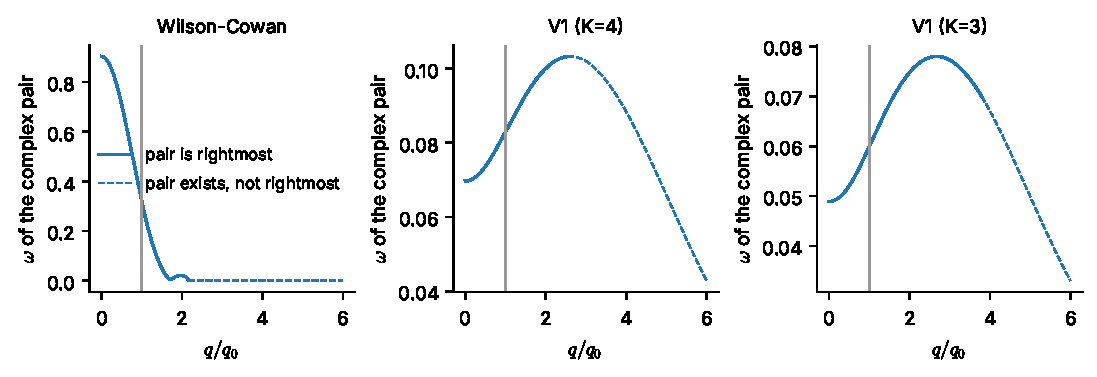
\includegraphics[width=\textwidth]{../../figures/dispersion_bell.pdf}
 \caption{Frequency of the complex pair at onset versus $q/q_0$. Solid: the
 pair is the rightmost eigenvalue. Dashed: the pair exists but another
 eigenvalue is to its right. The vertical line marks $q_0$.}
 \label{fig:dispersion-bell}
\end{figure}

\paragraph{Why the shape matters.}
A uniform input at frequency $\Omega$ is resonant with the modes that satisfy
$2\omega(q)=\Omega$. On a monotone branch there is one such $q$, so a faster
flicker selects a finer (V1) or a coarser (Wilson--Cowan) pattern. On a bell
there can be two such $q$, and none above $2\max\omega$. This is an
observation about the linear resonance condition only; on the torus only
the lattice values $q=2\pi h/L$ are available.

\section{Forcing strength and wavenumber}
\label{sec:forcing-strength}
Sections 5--7 used the resonant inputs
$2\omega_0$ and $2k_0$ at order $\epsilon^2$. Here we ask what happens for a
static input at any other wavenumber $k$, and how weak it may be. The answer
follows from one counting rule.

\subsection{Counting rule}
Take the static input $\epsilon^m(S\ee^{\ii kx}+\overline S\ee^{-\ii kx})$,
$k\in\NN$, and $p=\epsilon^2\mu$. Its response is
$s_k\ee^{\ii kx}+\cc$ with $s_k=R(0,k)S$, as in \eqref{eq:forcing-responses}.
This response exists for every $k$ because the critical modes oscillate,
$\omega_0\neq0$. The input
changes the amplitude equations only through terms that are resonant with
$E_+$. With $r$ factors of the input and one critical wave, the wave types are
\begin{equation*}
\begin{array}{c|c|c}
 r & \text{wave types} & \text{resonant with }E_+\text{ when}\\ \hline
 1 & (\omega_0,\ \pm k_0\pm k) & k=0\ \text{or}\ k=2k_0\\
 2 & (\omega_0,\ \pm k_0\pm k\pm k) & \text{always }(k-k=0),\ \text{and }k=k_0
\end{array}
\end{equation*}
A term with $r$ factors has order $\epsilon^{rm+1}$. It must meet $a\,A$ at
order $\epsilon^3$. Hence
\begin{equation}
 \boxed{k=2k_0:\ m=2,\ \ \text{input}\propto\epsilon^2;\qquad
 k\notin\{0,2k_0\}:\ m=1,\ \ \text{input}\propto\epsilon.}
 \label{eq:forcing-scaling}
\end{equation}
Section~2.3 excluded $m=1$ to keep $u_1$ in $\ker\cD$. For a non-resonant
input, the extra term $s_k\ee^{\ii kx}$ in $u_1$ is a forced response, not
a free amplitude, so $m=1$ is admissible. The same counting for a uniform
input at frequency $\omega$ gives $\omega\in\{0,2\omega_0\}$ with one factor,
and $\omega=\omega_0$ or any $\omega$ with two factors (unchecked: we have not
computed these coefficients). The table stops at $r=2$, that is, at order
$\epsilon^3$. With $r$ factors, $rk=2k_0$ is resonant at a higher order.

\subsection{Amplitude equations for $m=1$}
Let $k\notin\{0,2k_0\}$ and $S$ real. At order $\epsilon^3$ the input
contributes $A\,\chi$ for every $k$, and $B\,\xi$ only for $k=k_0$:
\begin{subequations}
\label{eq:static-amplitude}
\begin{align}
 A_\tau&=A\left(a+\chi+b|A|^2+c|B|^2\right)+\xi B,\\
 B_\tau&=B\left(a+\chi+b|B|^2+c|A|^2\right)+\xi A.
\end{align}
\end{subequations}
Here $\cC$ acts pointwise, as in the field \eqref{eq:population-field}. The
coefficients collect the second-order responses, as in \eqref{eq:G-vectors}:
\begin{align}
 \chi&=\Psi^*\Bigl[2\cQ\bigl(\Phi,2R(0,0)\cQ(s_k,\overline{s_k})\bigr)
 +4\cQ\bigl(\overline{s_k},R(\omega_0,k_0+k)\cQ(\Phi,s_k)\bigr)\notag\\
 &\qquad+4\cQ\bigl(s_k,R(\omega_0,k_0-k)\cQ(\Phi,\overline{s_k})\bigr)
 +6\cC(\Phi,s_k,\overline{s_k})\Bigr],\notag\\
 \xi&=\one{k=k_0}\Psi^*\Bigl[2\cQ\bigl(\Phi,R(0,2k_0)\cQ(s_k,s_k)\bigr)
 +4\cQ\bigl(s_k,R(\omega_0,0)\cQ(\Phi,s_k)\bigr)
 +3\cC(\Phi,s_k,s_k)\Bigr].
 \label{eq:chi-xi}
\end{align}
Both are quadratic in the input. At $A=B=0$ the combinations $A\pm B$
decouple with growth rates $\RePart(\mu\alpha+\chi\pm\xi)$. For $k=2k_0$,
Section~6 gives $\RePart(\mu\alpha\pm\eta_x)$ instead. Write the input as a
cosine of peak $\delta$. With $\RePart\alpha>0$ \eqref{eq:transversality}, the
threshold moves to
\begin{equation}
 \boxed{p_{\rm th}=-\frac{\RePart\chi^{(1)}+|\RePart\xi^{(1)}|}{\RePart\alpha}\,\delta^2
 \quad(k\notin\{0,2k_0\}),\qquad
 p_{\rm th}=-\frac{|\RePart\eta_x^{(1)}|}{\RePart\alpha}\,|\delta|
 \quad(k=2k_0),}
 \label{eq:threshold-shift}
\end{equation}
where the superscript $(1)$ marks the value for $\delta=1$. At this order
only $k=k_0$ and $k=2k_0$ lock the pattern to the input. Every other $k$ moves
the threshold but leaves the spatial phase free.

\subsection{The two-parameter diagram}
Figure~\ref{fig:two-parameter} repeats the $(\delta,a_{EE})$ diagram for the E--I
Wilson--Cowan model on $L=60$ ($k_0=3$). For each stimulus wavenumber $k$ it
shows the $a_{EE}$ at which the stimulus-locked steady state first loses
stability. Near $\delta=0$, \eqref{eq:threshold-shift} explains the two shapes.
\begin{itemize}
 \item $k=6=2k_0$: the two branches $A=\pm B$ are straight lines with slopes
 $\pm22.26$ that cross at $\delta=0$. The threshold is a V. A continuation that
 follows one Hopf branch through $\delta=0$ traces one line across the other,
 which gives the loop.
 \item $k\le3$: both branches are parabolas tangent at $\delta=0$, so the curve
 is smooth there.
\end{itemize}
The quadratic coefficients and a check against the full model at small $q$
are (shifts in units of $10^{-4}$)
\begin{equation*}
\begin{array}{c|cccccc}
 k & 1 & 2 & 3\,(=k_0) & 4 & 5 & 6\,(=2k_0)\\ \hline
 \text{coefficient of }\delta^2\text{ or }|\delta| & 3.38 & 5.32 & 13.9 & 662 & 2032 & -22.26\\
 \text{shift, full model} & 0.84 & 1.32 & 3.48 & 26.6 & 82.2 & -437\\
 \text{shift, theory} & 0.84 & 1.33 & 3.48 & 26.5 & 81.3 & -445
\end{array}
\end{equation*}
with $\delta=0.005$ for $k\le3$ and $\delta=0.002$ otherwise. Near
$\delta=0$, every $k$ except $2k_0$ raises the threshold. The coefficients for $m=4,5$ are large
because $R(0,k)$ is large there. These modes have eigenvalues close to zero,
$-0.025+0.115\ii$ and $-0.084+0.009\ii$, which is the falling frequency curve
of Section~\ref{sec:frequency-shape}. Their quadratic range is therefore
small, $|\delta|\lesssim0.002$. Far from $\delta=0$ all curves bend down,
outside the weakly nonlinear range.

\begin{figure}[h]
 \centering
 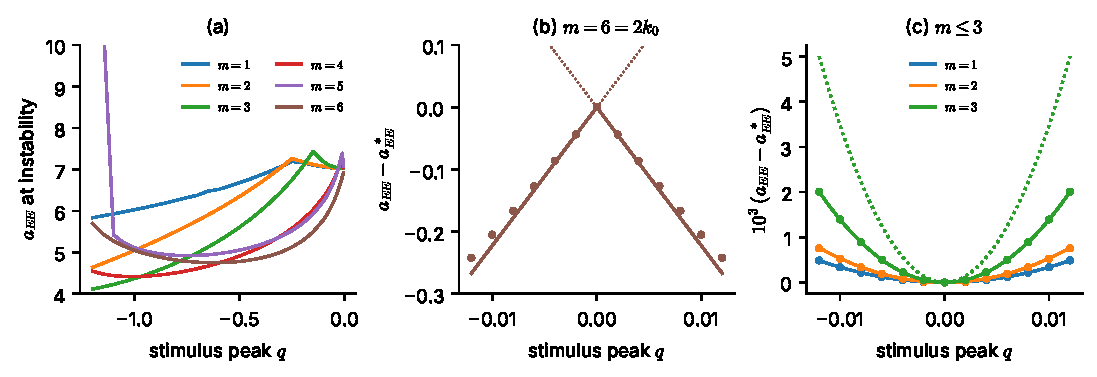
\includegraphics[width=\textwidth]{../../figures/two_parameter_curves.pdf}
 \caption{Static stimulus $\delta\cos(2\pi kx/60)$ on E, Wilson--Cowan, $N=60$.
 (a) $a_{EE}$ at the first instability of the stimulus-locked state.
 (b), (c) the same near $\delta=0$: dots from the full model, lines from
 \eqref{eq:threshold-shift}, dotted lines for the second branch.}
 \label{fig:two-parameter}
\end{figure}

\section{Two dimensions}
\label{sec:two-dimensions}
On the square torus $\T_L^2$ the critical modes form a shell: all lattice
wavevectors $\boldsymbol k$ with $|\boldsymbol k|=q_0$. Each gives a wave
$E_{\boldsymbol k}=\ee^{\ii(\omega_0s+\boldsymbol k\cdot\boldsymbol x)}$ with
amplitude $A_{\boldsymbol k}$, and
$u_1=\sum_{\boldsymbol k}A_{\boldsymbol k}\Phi E_{\boldsymbol k}+\cc$
The 1D amplitudes are $A=A_{k_0\hat x}$ and $B=A_{-k_0\hat x}$. We use three
assumptions.
\begin{assumption}\label{as:isotropy}
$M_0$, $\cQ$ and $\cC$ depend on a wavevector only through its length (true
for the field \eqref{eq:population-field} with isotropic Gaussian kernels), and
$\cC$ acts pointwise.
\end{assumption}
\begin{assumption}\label{as:one-shell}
At $p=0$ only the shell $|\boldsymbol k|=q_0$ has eigenvalues on the imaginary
axis, the pair $\pm\ii\omega_0$; all other lattice modes are strictly stable.
\end{assumption}
\begin{assumption}\label{as:2d-nonresonance}
For all shell waves, $2\ii\omega_0\notin\operatorname{spec}M_0(|\boldsymbol k_X+\boldsymbol k_Z|)$
and $0\notin\operatorname{spec}M_0(|\boldsymbol k_X-\boldsymbol k_Y|)$ unless the
difference is zero; for an input $\boldsymbol K$ at $\Omega=2\omega_0$, also
$2\ii\omega_0\notin\operatorname{spec}M_0(|\boldsymbol K|)$.
\end{assumption}
Assumption~\ref{as:2d-nonresonance} replaces \eqref{eq:no-quadratic-resonance}.
Under these assumptions the calculation of Sections~3--5 carries over word for
word; only the bookkeeping of wavevectors changes.

\subsection{Which waves an input couples}
Take an input $\epsilon^2(H\ee^{\ii(\Omega t+\boldsymbol K\cdot\boldsymbol x)}+\cc)$.
At order $\epsilon^3$ it couples two critical waves when their wave types add
up, exactly as in \eqref{eq:temporal-critical-A}--\eqref{eq:spatial-critical-B}:
\begin{equation}
\begin{array}{c|c|c}
 \text{input} & \text{coupled waves} & \text{term in } (A_{\boldsymbol k_Y})_\tau\\ \hline
 \Omega=2\omega_0 & \boldsymbol k_X+\boldsymbol k_Y=\boldsymbol K &
 \eta(|\boldsymbol K|)\,\overline{A_{\boldsymbol k_X}},\quad
 \eta(K)=2\Psi^*\cQ\bigl(\overline\Phi,R(2\omega_0,K)H\bigr)\\
 \Omega=0 & \boldsymbol k_Y-\boldsymbol k_X=\pm\boldsymbol K &
 \eta_s^\pm\,A_{\boldsymbol k_X},\quad
 \eta_s^+=2\Psi^*\cQ\bigl(\Phi,R(0,K)H\bigr),\ \
 \eta_s^-=2\Psi^*\cQ\bigl(\Phi,R(0,K)\overline H\bigr)
\end{array}
\label{eq:wavevector-rule}
\end{equation}
Here $K=|\boldsymbol K|$; the $-\boldsymbol K$ row comes from the complex
conjugate of the input. For $\boldsymbol K=0$ and $\Omega=2\omega_0$ this is
$\eta_t$; for $K=2k_0$ and $\Omega=0$ it gives $\eta_\pm$.

\paragraph{Geometry.}
Both coupled waves have length $q_0$. For $\Omega=2\omega_0$ they are
therefore placed symmetrically about $\boldsymbol K$:
\begin{equation}
 \boldsymbol k_{X,Y}=\tfrac12\boldsymbol K\pm\boldsymbol d,\qquad
 \boldsymbol d\perp\boldsymbol K,\qquad
 |\boldsymbol d|^2=q_0^2-\tfrac14|\boldsymbol K|^2.
 \label{eq:pair-geometry}
\end{equation}
There are three cases.
\begin{itemize}
 \item $\boldsymbol K=0$ (uniform flicker): each wave couples to its
 opposite. No direction is preferred.
 \item $|\boldsymbol K|=2q_0$: $\boldsymbol d=0$ and the wave couples to
 itself. A traveling input selects one traveling wave along
 $\boldsymbol K$.
 \item $0<|\boldsymbol K|<2q_0$: the pair has a component $\pm\boldsymbol d$
 across $\boldsymbol K$. An input traveling along $x$ then creates
 structure along $y$.
\end{itemize}
On the torus, $\boldsymbol k_{X,Y}$ must be lattice vectors. On the axial
shell $\{(\pm k_0,0),(0,\pm k_0)\}$, an input along an axis can only have
$K\in\{0,2q_0\}$, so it produces no structure across itself; the diagonal input
$\boldsymbol K=(k_0,k_0)$ couples $(k_0,0)$ with $(0,k_0)$. On the oblique shell
$\{(\pm3,\pm1),(\pm1,\pm3)\}$ the axial input $\boldsymbol K=(6,0)$ couples
$(3,1)$ with $(3,-1)$.

\subsection{Cubic terms}
The cubic terms are found as in Section~5. The equation of
$A_{\boldsymbol k}$ contains every monomial
$A_{\boldsymbol k_X}\overline{A_{\boldsymbol k_Y}}A_{\boldsymbol k_Z}$ with
$\boldsymbol k_X-\boldsymbol k_Y+\boldsymbol k_Z=\boldsymbol k$. For distinct
$\boldsymbol k_X\neq\boldsymbol k_Z$, its coefficient is
\begin{equation}
 \boxed{\Psi^*\Bigl[2\cQ\bigl(\Phi,h_{11}(\boldsymbol k_X-\boldsymbol k_Y)\bigr)
 +2\cQ\bigl(\overline\Phi,h_{20}(\boldsymbol k_X+\boldsymbol k_Z)\bigr)
 +2\cQ\bigl(\Phi,h_{11}(\boldsymbol k_Z-\boldsymbol k_Y)\bigr)
 +6\cC(\Phi,\Phi,\overline\Phi)\Bigr],}
 \label{eq:general-cubic}
\end{equation}
with $h_{20}(\boldsymbol v)=2R(2\omega_0,|\boldsymbol v|)\cQ(\Phi,\Phi)$ and
$h_{11}(\boldsymbol v)=2R(0,|\boldsymbol v|)\cQ(\Phi,\overline\Phi)$. Each
term is one pair of waves forming a second-order response, then meeting the
third wave. For $\boldsymbol k_X=\boldsymbol k_Z$ (the monomial
$A_{\boldsymbol k_X}^2\overline{A_{\boldsymbol k_Y}}$) each multiplicity halves:
\begin{equation}
 \Psi^*\Bigl[\cQ\bigl(\overline\Phi,h_{20}(2\boldsymbol k_X)\bigr)
 +2\cQ\bigl(\Phi,h_{11}(\boldsymbol k_X-\boldsymbol k_Y)\bigr)
 +3\cC(\Phi,\Phi,\overline\Phi)\Bigr],
 \label{eq:general-cubic-repeated}
\end{equation}
and $\boldsymbol k_X=\boldsymbol k_Y=\boldsymbol k_Z$ gives $b$ \eqref{eq:Gs}.
Two further cases recur.
\begin{itemize}
 \item Two waves at angle $\theta\neq0$
 ($\boldsymbol k_Y=\boldsymbol k_Z$): the cross coefficient $c_\theta$, whose
 responses sit at $|\boldsymbol k_X\pm\boldsymbol k_Y|=2q_0|\cos\frac\theta2|$
 and $2q_0|\sin\frac\theta2|$. It gives $c_\pi=c$ and $c_{\pi/2}=c_\perp$.
 \item Four waves of the axial shell: the quartet term
 $c_\times\overline{A_{-\hat x}}A_{\hat y}A_{-\hat y}$ in the
 $A_{\hat x}$ equation (lattice directions in units of $k_0$).
\end{itemize}

\subsection{The locked pair}
\begin{proposition}
Assume \ref{as:isotropy}--\ref{as:2d-nonresonance}. Let an input with
$\Omega=2\omega_0$ couple the pair $\boldsymbol k_X\neq\boldsymbol k_Y$ of
\eqref{eq:pair-geometry}, at angle $\theta$, and assume that no shell wave
equals $2\boldsymbol k_X-\boldsymbol k_Y$ or $2\boldsymbol k_Y-\boldsymbol k_X$.
Then $A_{\boldsymbol k_X}=A_{\boldsymbol k_Y}=z$ with all other amplitudes zero
is invariant, and
\begin{equation}
 z_\tau=z\bigl(a+(b+c_\theta)|z|^2\bigr)+\eta\,\overline z .
 \label{eq:pair-reduction}
\end{equation}
This is \eqref{eq:standing-reduction} with $a_+=a$ and $\gamma=b+c_\theta$.
If $b+c_\theta\neq0$ and $|\eta|>|\mu\alpha|$, Proposition~1 gives
$z_*=\sqrt{\rho_*}\ee^{\ii\phi_*}$
and the leading field
\begin{equation}
 \boxed{u=4\epsilon\sqrt{\rho_*}\,
 \RePart\!\left[\Phi\ee^{\ii(\omega_0t+\frac12\boldsymbol K\cdot\boldsymbol x+\phi_*)}\right]
 \cos(\boldsymbol d\cdot\boldsymbol x)+O(\epsilon^2).}
 \label{eq:pair-field}
\end{equation}
\end{proposition}
\begin{proof}
On the subspace, the monomials that contain only $A_{\boldsymbol k_X}$ and
$A_{\boldsymbol k_Y}$ land on $\boldsymbol k_X$, $\boldsymbol k_Y$,
$2\boldsymbol k_X-\boldsymbol k_Y$, or $2\boldsymbol k_Y-\boldsymbol k_X$. By
assumption the last two are not shell waves, so all other amplitudes stay
zero. An input term $\eta\overline{A_{\boldsymbol k_{X'}}}$ is nonzero on the
subspace only if $\boldsymbol k_{X'}\in\{\boldsymbol k_X,\boldsymbol k_Y\}$, and
then it lands on $\boldsymbol K-\boldsymbol k_{X'}\in\{\boldsymbol k_Y,\boldsymbol k_X\}$.
The $A_{\boldsymbol k_X}$ equation contains
$b|A_{\boldsymbol k_X}|^2$, $c_\theta|A_{\boldsymbol k_Y}|^2$, and, by
\eqref{eq:wavevector-rule}, $\eta\overline{A_{\boldsymbol k_Y}}$. The
$A_{\boldsymbol k_Y}$ equation is the same with $X$ and $Y$ exchanged, which
gives \eqref{eq:pair-reduction}. Finally
$\ee^{\ii\boldsymbol k_X\cdot\boldsymbol x}+\ee^{\ii\boldsymbol k_Y\cdot\boldsymbol x}
=2\ee^{\ii\boldsymbol K\cdot\boldsymbol x/2}\cos(\boldsymbol d\cdot\boldsymbol x)$.
\end{proof}
For $\boldsymbol K=0$ this is the 1D standing pattern \eqref{eq:below-onset-pattern};
the perpendicular pair is also driven but stays zero on the subspace.
For $0<|\boldsymbol K|<2q_0$ the pattern travels with the input along
$\boldsymbol K$ and is standing across it, with wavenumber
$|\boldsymbol d|=(q_0^2-|\boldsymbol K|^2/4)^{1/2}$ set by the input. An
input traveling along $x$ thus creates a spatial pattern along $y$. A static
input ($\Omega=0$) couples $\boldsymbol k_Y=\boldsymbol k_X+\boldsymbol K$
instead, which gives a pattern standing along $\boldsymbol K$ and traveling
across it; we do not treat it further.

\subsection{Stability inside the shell}
The pair is stable in the whole problem only if the other shell waves decay.
Their linearized growth involves $c_\theta$ at the angles to
$\boldsymbol k_X$ and $\boldsymbol k_Y$, and the four-wave terms of
\eqref{eq:general-cubic}. For uniform flicker on the axial shell this is
explicit. At the stripe $A_{\pm\hat x}=z_*$, the perpendicular pair obeys
$v_\tau=hv+\ell\,\overline w$ with
\begin{equation}
 h=a+2c_\perp\rho_*,\qquad \ell=\eta_t+c_\times\rho_*\ee^{2\ii\phi_*},\qquad
 \boxed{\lambda_\perp=\RePart\Bigl[h+\sqrt{|\ell|^2-(\operatorname{Im}h)^2}\Bigr],}
 \label{eq:stripe-transverse}
\end{equation}
so the stripe is stable across $x$ when $\RePart h<0$ and $|\ell|<|h|$. The
square $A_{\pm\hat x}=A_{\pm\hat y}=z$ obeys \eqref{eq:pair-reduction} with
$b+c_\theta$ replaced by $\gamma_\square=b+c+2c_\perp+c_\times$. For other
shells we evaluate the full Jacobian numerically.

The sign of $\RePart c_\theta$ decides the outcome. In V1 it is negative at
every angle. In the E--I model it is positive for
$71^\circ\lesssim\theta\lesssim146^\circ$ (Figure~\ref{fig:cross-coupling}).
There, one wave amplifies another. A pattern destabilizes when the shell holds
waves at such angles to it, and the cubic equations then cannot saturate.
The sharp peak near $141^\circ$ is a near resonance. There the sum of the two
wavevectors has length $0.67q_0$, where $M$ has eigenvalues
$-0.039\pm0.566\ii$, close to $2\omega_0=0.593$, so $R(2\omega_0,\cdot)$ is
large. This is the falling frequency curve of
Section~\ref{sec:frequency-shape} again: in the E--I model a longer wave
oscillates faster and can match $2\omega_0$.

\begin{figure}[h]
 \centering
 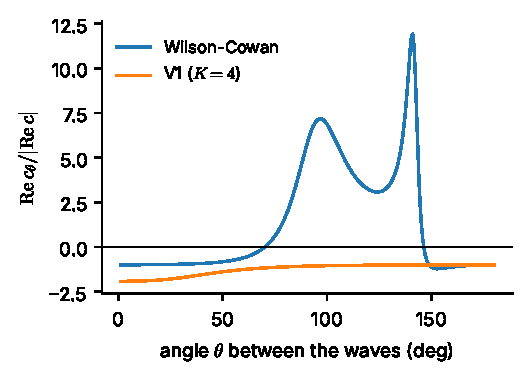
\includegraphics[width=.5\textwidth]{../../figures/cross_coupling.pdf}
 \caption{$\RePart c_\theta$ against the angle between two critical waves,
 scaled by $|\RePart c|$. Wilson--Cowan on $L=58.26$ (axial shell critical)
 and V1 on $L=43$.}
 \label{fig:cross-coupling}
\end{figure}

\subsection{Numerical tests}
\label{sec:2d-tests}
We integrate the full 2D field below onset ($\mu=-1$, $32\times32$ grid) and
measure the amplitudes of the shell waves. The domain length is chosen so
that the intended shell is critical: $L=58.26$ (axial) and $L=61.42$
(oblique) for Wilson--Cowan, and $L=43$ and $L=45.01$ for V1.
{\small
\begin{equation*}
\begin{array}{l|l|cc}
 \text{test} & \text{model, }\epsilon & \text{direct field} & \text{theory}\\ \hline
 y\text{-wave growth }\RePart(\mu\alpha+c_\perp\rho_T) & \text{WC, }0.1 & +0.588 & +0.557\\
 & \text{V1, }0.05\ /\ 0.025 & -0.0080\ /\ -0.0098 & -0.0103\\
 \text{flicker: stripe amplitude} & \text{WC, }0.1 & 0.02389 & 0.02385\\
 & \text{V1, }0.05\ /\ 0.025 & 0.00378\ /\ 0.00196 & 0.00409\ /\ 0.00204\\
 \text{flicker: stripe }\lambda_\perp & \text{WC, }0.1 & +1.77 & +1.84\\
 & \text{V1, }0.05\ /\ 0.025 & -0.017\ /\ -0.024 & -0.026\\
 \text{flicker: square amplitude} & \text{V1, }0.05\ /\ 0.025 & 0.00256\ /\ 0.001373 & 0.00276\ /\ 0.001378\\
 x\text{-traveling input: pair }|A| & \text{WC, }0.1 & 0.0264\ \text{(then leaves)} & 0.0270\ \text{(unstable)}\\
 & \text{V1, }0.05\ /\ 0.025 & 0.00397\ /\ 0.00242 & 0.00509\ /\ 0.00254\ \text{(stable)}
\end{array}
\end{equation*}}
The first test runs above onset ($\mu=+1$) on the traveling wave $A_{\hat x}$ of
size $\rho_T=-\RePart\alpha/\RePart b$; rates are per slow time. In every V1 test the gap shrinks when $\epsilon$ is
halved, as expected for $O(\epsilon)$ corrections. In V1 the stripe under flicker is
stable across $x$, while the square is unstable to a symmetry-breaking mode
($+0.022$). In the E--I model both are unstable: the stripe across $x$, and
the square inside its own subspace ($+0.236$). Under the $x$-traveling input
on the oblique shell, the pair $(3,\pm1)$ is selected from noise in both
models, and the other six waves stay below $10^{-5}$. In V1 it persists. In
the E--I model the waves $(\pm1,\pm3)$ grow, at the predicted rate $+0.59$,
once the pair is near $z_*$. The field then leaves the weakly nonlinear range.

\subsection{Summary}
The 2D picture has three steps. The input wavevector selects which critical
waves are coupled \eqref{eq:wavevector-rule}. The coupled pair is a 1D
problem, and Proposition~1 gives its amplitude \eqref{eq:pair-reduction}.
The cross coefficients $c_\theta$ then decide whether that pair survives the
rest of the shell. The multi-population V1 model passes the third step. The
two-population E--I model with these parameters fails it: its perpendicular
coupling is destabilizing.

\subsection{Notation for Sections 8.4--10}
\begingroup\small
\noindent\begin{tabular}{@{}p{0.19\textwidth}p{0.6\textwidth}p{0.14\textwidth}@{}}
\toprule
Symbol & Definition & Location\\
\midrule
$s_k,\delta$ & static response $R(0,k)S$ to an order-$\epsilon$ input; cosine peak of the input & Sec.~9\\
$\chi,\xi$ & input-induced shift and $A$--$B$ coupling for $m=1$ & \eqref{eq:chi-xi}\\
$E_{\boldsymbol k},A_{\boldsymbol k}$ & critical wave $\ee^{\ii(\omega_0t+\boldsymbol k\cdot\boldsymbol x)}$ and its amplitude, $|\boldsymbol k|=q_0$ & Sec.~10\\
$\boldsymbol K,\eta(K),\eta_s^\pm$ & input wavevector; coupling of a pair at $\Omega=2\omega_0$ or $\Omega=0$ & \eqref{eq:wavevector-rule}\\
$\boldsymbol d$ & half difference of the coupled pair, $\perp\boldsymbol K$ & \eqref{eq:pair-geometry}\\
$c_\theta,c_\perp,c_\times$ & cross coefficient at angle $\theta$; $c_\perp=c_{\pi/2}$; axial quartet coefficient & \eqref{eq:general-cubic}\\
$\gamma_\square,\lambda_\perp$ & square coefficient $b+c+2c_\perp+c_\times$; transverse growth of the stripe & \eqref{eq:stripe-transverse}\\
\bottomrule
\end{tabular}
\endgroup

\clearpage
\begin{thebibliography}{4}
\bibitem{pfeffer2013}
C.~K. Pfeffer, M. Xue, M. He, Z.~J. Huang, and M. Scanziani.
Inhibition of inhibition in visual cortex: the logic of connections between
molecularly distinct interneurons.
\emph{Nature Neuroscience} 16 (2013), 1068--1076.
\href{https://doi.org/10.1038/nn.3446}{doi:10.1038/nn.3446}.

\bibitem{billeh2020}
Y.~N. Billeh et al.
Systematic Integration of Structural and Functional Data into Multi-scale
Models of Mouse Primary Visual Cortex.
\emph{Neuron} 106 (2020), 388--403.e18; Fig.~4 and STAR Methods.
\href{https://doi.org/10.1016/j.neuron.2020.01.040}{doi:10.1016/j.neuron.2020.01.040}.

\bibitem{campagnola2022}
L. Campagnola et al.
Local connectivity and synaptic dynamics in mouse and human neocortex.
\emph{Science} 375 (2022), eabj5861.
\href{https://doi.org/10.1126/science.abj5861}{doi:10.1126/science.abj5861}.

\bibitem{ji2016}
X.-Y. Ji et al.
Thalamocortical Innervation Pattern in Mouse Auditory and Visual Cortex:
Laminar and Cell-Type Specificity.
\emph{Cerebral Cortex} 26 (2016), 2612--2625.
\href{https://doi.org/10.1093/cercor/bhv099}{doi:10.1093/cercor/bhv099}.
\end{thebibliography}

\end{document}
